\documentclass{article} % A4 paper and 11pt font size
\setcounter{secnumdepth}{0}

\usepackage{amssymb, amsmath, amsfonts}
\usepackage{moreverb}
\usepackage{multicol}
\usepackage{graphicx}
\usepackage{enumerate}
\usepackage{caption}
\usepackage{nicefrac}
\usepackage{graphics}
\usepackage[margin=1in]{geometry}
\usepackage{tocloft}
\renewcommand{\cftsecleader}{\cftdotfill{\cftdotsep}}
\usepackage{array}
\usepackage{arydshln}
\usepackage{float}
\usepackage{subcaption}
\usepackage{csquotes}
\usepackage{placeins}
\usepackage{verbatim}
\usepackage{hyperref}
\usepackage{textcomp}
\usepackage[makeroom]{cancel}
\usepackage{bbold}
\usepackage{scrextend}
\usepackage{alltt}
\usepackage[utf8]{inputenc}
\usepackage{listings}
\usepackage{color}
\usepackage{physics}
\usepackage{mathtools}
\usepackage[normalem]{ulem}
\usepackage{amsthm}
\usepackage{tikz}
\usetikzlibrary{positioning}
\usetikzlibrary{arrows}
\usepackage{pgfplots}
\usepackage{bigints}
\allowdisplaybreaks
\pgfplotsset{compat=1.12}

\theoremstyle{plain}
\newtheorem*{theorem*}{Theorem}
\newtheorem{theorem}{Theorem}
\newtheorem*{lemma*}{Lemma}
\newtheorem{lemma}{Lemma}

\definecolor{verbgray}{gray}{0.9}
% \definecolor{dkgreen}{green}{0.9}

\lstdefinestyle{PythonCode}{%
  language=Python,
  backgroundcolor=\color{verbgray},
  keywordstyle=\color{blue},      % keyword style
  keywordstyle=[2]\color{blue},   % keyword style
  commentstyle=\color{magenta},   % comment style
  stringstyle=\color{olive},      % string literal styleframe=single,
  numberstyle=\color{black},      % string literal styleframe=single,
  framerule=0pt,
  numbers=left,
  stepnumber=1,
  firstnumber=1,
  showspaces=false,
  basicstyle=\ttfamily}

\lstset{style=PythonCode}

\makeatletter
\newcommand{\BIGG}{\bBigg@{3}}
\newcommand{\vast}{\bBigg@{4}}
\newcommand{\Vast}{\bBigg@{5}}
\makeatother

\newenvironment{definition}[1][Definition]{\begin{trivlist}
\item[\hskip \labelsep {\bfseries #1}]}{\end{trivlist}}

\newcommand{\dy}{\partial_y}
\newcommand{\dyy}{\partial_{yy}}
\newcommand{\dxx}{\partial_{xx}}
\newcommand{\dxy}{\partial_{xy}}
\newcommand{\dyyy}{\partial_{yyy}}
\newcommand{\dxxx}{\partial_{xxx}}
\newcommand{\dx}{\partial_x}
\newcommand{\E}{\varepsilon}
\def\Rl{\mathbb{R}}
\def\Cx{\mathbb{C}}

\newcommand{\Ei}{\text{Ei}}

\usepackage[T1]{fontenc} % Use 8-bit encoding that has 256 glyphs
\usepackage{fourier} % Use the Adobe Utopia font for the document - comment this line to return to the LaTeX default
\usepackage[english]{babel} % English language/hyphenation

\usepackage{sectsty} % Allows customizing section commands
\allsectionsfont{\centering \normalfont\scshape} % Make all sections centered, the default font and small caps

\usepackage{fancyhdr} % Custom headers and footers
\pagestyle{fancy} % Makes all pages in the document conform to the custom headers and footers
\fancyhead[L]{\bf Sam Fleischer}
\fancyhead[C]{\bf UC Davis \\ Numerical Solutions of Differential Equations (MAT228A)} % No page header - if you want one, create it in the same way as the footers below
\fancyhead[R]{\bf Fall 2016}

\fancyfoot[L]{\bf } % Empty left footer
\fancyfoot[C]{\bf \thepage} % Empty center footer
\fancyfoot[R]{\bf } % Page numbering for right footer
\renewcommand{\headrulewidth}{0pt} % Remove header underlines
\renewcommand{\footrulewidth}{0pt} % Remove footer underlines
\setlength{\headheight}{25pt} % Customize the height of the header

\newcommand{\VEC}[2]{\left\langle #1, #2 \right\rangle}
\newcommand{\ran}{\text{\rm ran }}
\newcommand{\Hilb}{\mathcal{H}}
\newcommand{\lap}{\Delta}

\newcommand{\littleo}[1]{\text{\scriptsize$\mathcal{O}$}\qty(#1)}

\DeclareMathOperator*{\esssup}{\text{ess~sup}}

\newcommand{\problem}[2]{
\vspace{.375cm}
\boxed{\begin{minipage}{\textwidth}
    \section{\bf #1}
    #2
\end{minipage}}
}

\numberwithin{equation}{section} % Number equations within sections (i.e. 1.1, 1.2, 2.1, 2.2 instead of 1, 2, 3, 4)
\numberwithin{figure}{section} % Number figures within sections (i.e. 1.1, 1.2, 2.1, 2.2 instead of 1, 2, 3, 4)
\numberwithin{table}{section} % Number tables within sections (i.e. 1.1, 1.2, 2.1, 2.2 instead of 1, 2, 3, 4)

\setlength\parindent{0pt} % Removes all indentation from paragraphs - comment this line for an assignment with lots of text

\newcommand{\horrule}[1]{\rule{\linewidth}{#1}} % Create horizontal rule command with 1 argument of height

\title{ 
\normalfont \normalsize 
\textsc{UC Davis, Numerical Solutions of Differential Equations (MAT 228A), Fall 2016} \\ [25pt] % Your university, school and/or department name(s)
\horrule{2pt} \\[0.4cm] % Thin top horizontal rule
\Huge Homework \#4 \\ % The assignment title
\horrule{2pt} \\[0.5cm] % Thick bottom horizontal rule
}

\author{\huge Sam Fleischer} % Your name

\date{December 2, 2016} % Today's date or a custom date

\begin{document}\thispagestyle{empty}

\maketitle % Print the title

\makeatletter
\@starttoc{toc}
\makeatother

\pagebreak

\problem{Part I}{White a multigrid V-cycle code to solve the Poisson equation in two dimensions on the unit square with Dirichlet boundary conditions.  Use full weighting for restriction, bilinear interpolation for prolongation, and red-black Gauss-Seidel for smoothing. \\

\textbf{Note:} If you cannot get a V-cycle code working, write a simple code such as a 2-grid code.  You can also experiment in one dimension (do not use GSRB in 1D).  You may turn in one of these simplified codes for reduced credit.  You should state what your code does, and use your code for the assignment. \\

\begin{enumerate}[\ \ 1.]
    \item Use your V-cycle code to solve $$\laplacian u = -\exp[-\qty(x - 0.25)^2 - (y - 0.6)^2]$$ on the unit square $(0,1)\times(0,1)$ with homogeneous Dirichlet boundary conditions for different grid spaces.  How many steps of pre and postsmoothing did you use?  What tolerance did you use?  How many cycles did it take to converge?  Compare the amount of work needed to reach convergence with your solvers from Homework 3 taking into account how much work is involved in a V-cycle.
\end{enumerate}}

Rather than working with grids of size $2^n + 1$ for integers $n$ and include $0$s on the boundary, I chose to work with grids of size $2^n - 1$ for integers $n$.  My code (written in Python) only takes the interior points into account.  Here is my restriction operator:
\lstinputlisting[language=Python, firstline=8, lastline=34]{operators.py}
and here is my interpolation operator:
\lstinputlisting[language=Python, firstline=36, lastline=61]{operators.py}
Here is my Gauss-Seidel Red-Black code:
\lstinputlisting[language=Python, firstline=6, lastline=63]{smoothers.py}
Here is a simple function to get a mesh of size $2^n-1$:
\lstinputlisting[language=Python, firstline=5, lastline=17]{get_mesh.py}
Here is a function to generate a discrete Laplacian in 1D:
\lstinputlisting[language=Python, firstline=63, lastline=73]{operators.py}
And here is a function to cleverly generate the discrete Laplacian in 2D using Kronecker products:
\lstinputlisting[language=Python, firstline=75, lastline=90]{operators.py}
Here is a function to compute the residual:
\lstinputlisting[language=Python, firstline=92, lastline=105]{operators.py}
Here is a simple function to directly solve the system with Dirichlet boundary conditions when the grid size is $1$:
\lstinputlisting[language=Python, firstline=13, lastline=22]{V_cycle.py}
Finally, here is the V-cycle code:
\lstinputlisting[language=Python, firstline=24, lastline=72]{V_cycle.py}

Here are some results of the V-cycle code:
\begin{figure}[!htb]
    \centering
    \begin{subfigure}[b]{0.45\textwidth}
        \centering
        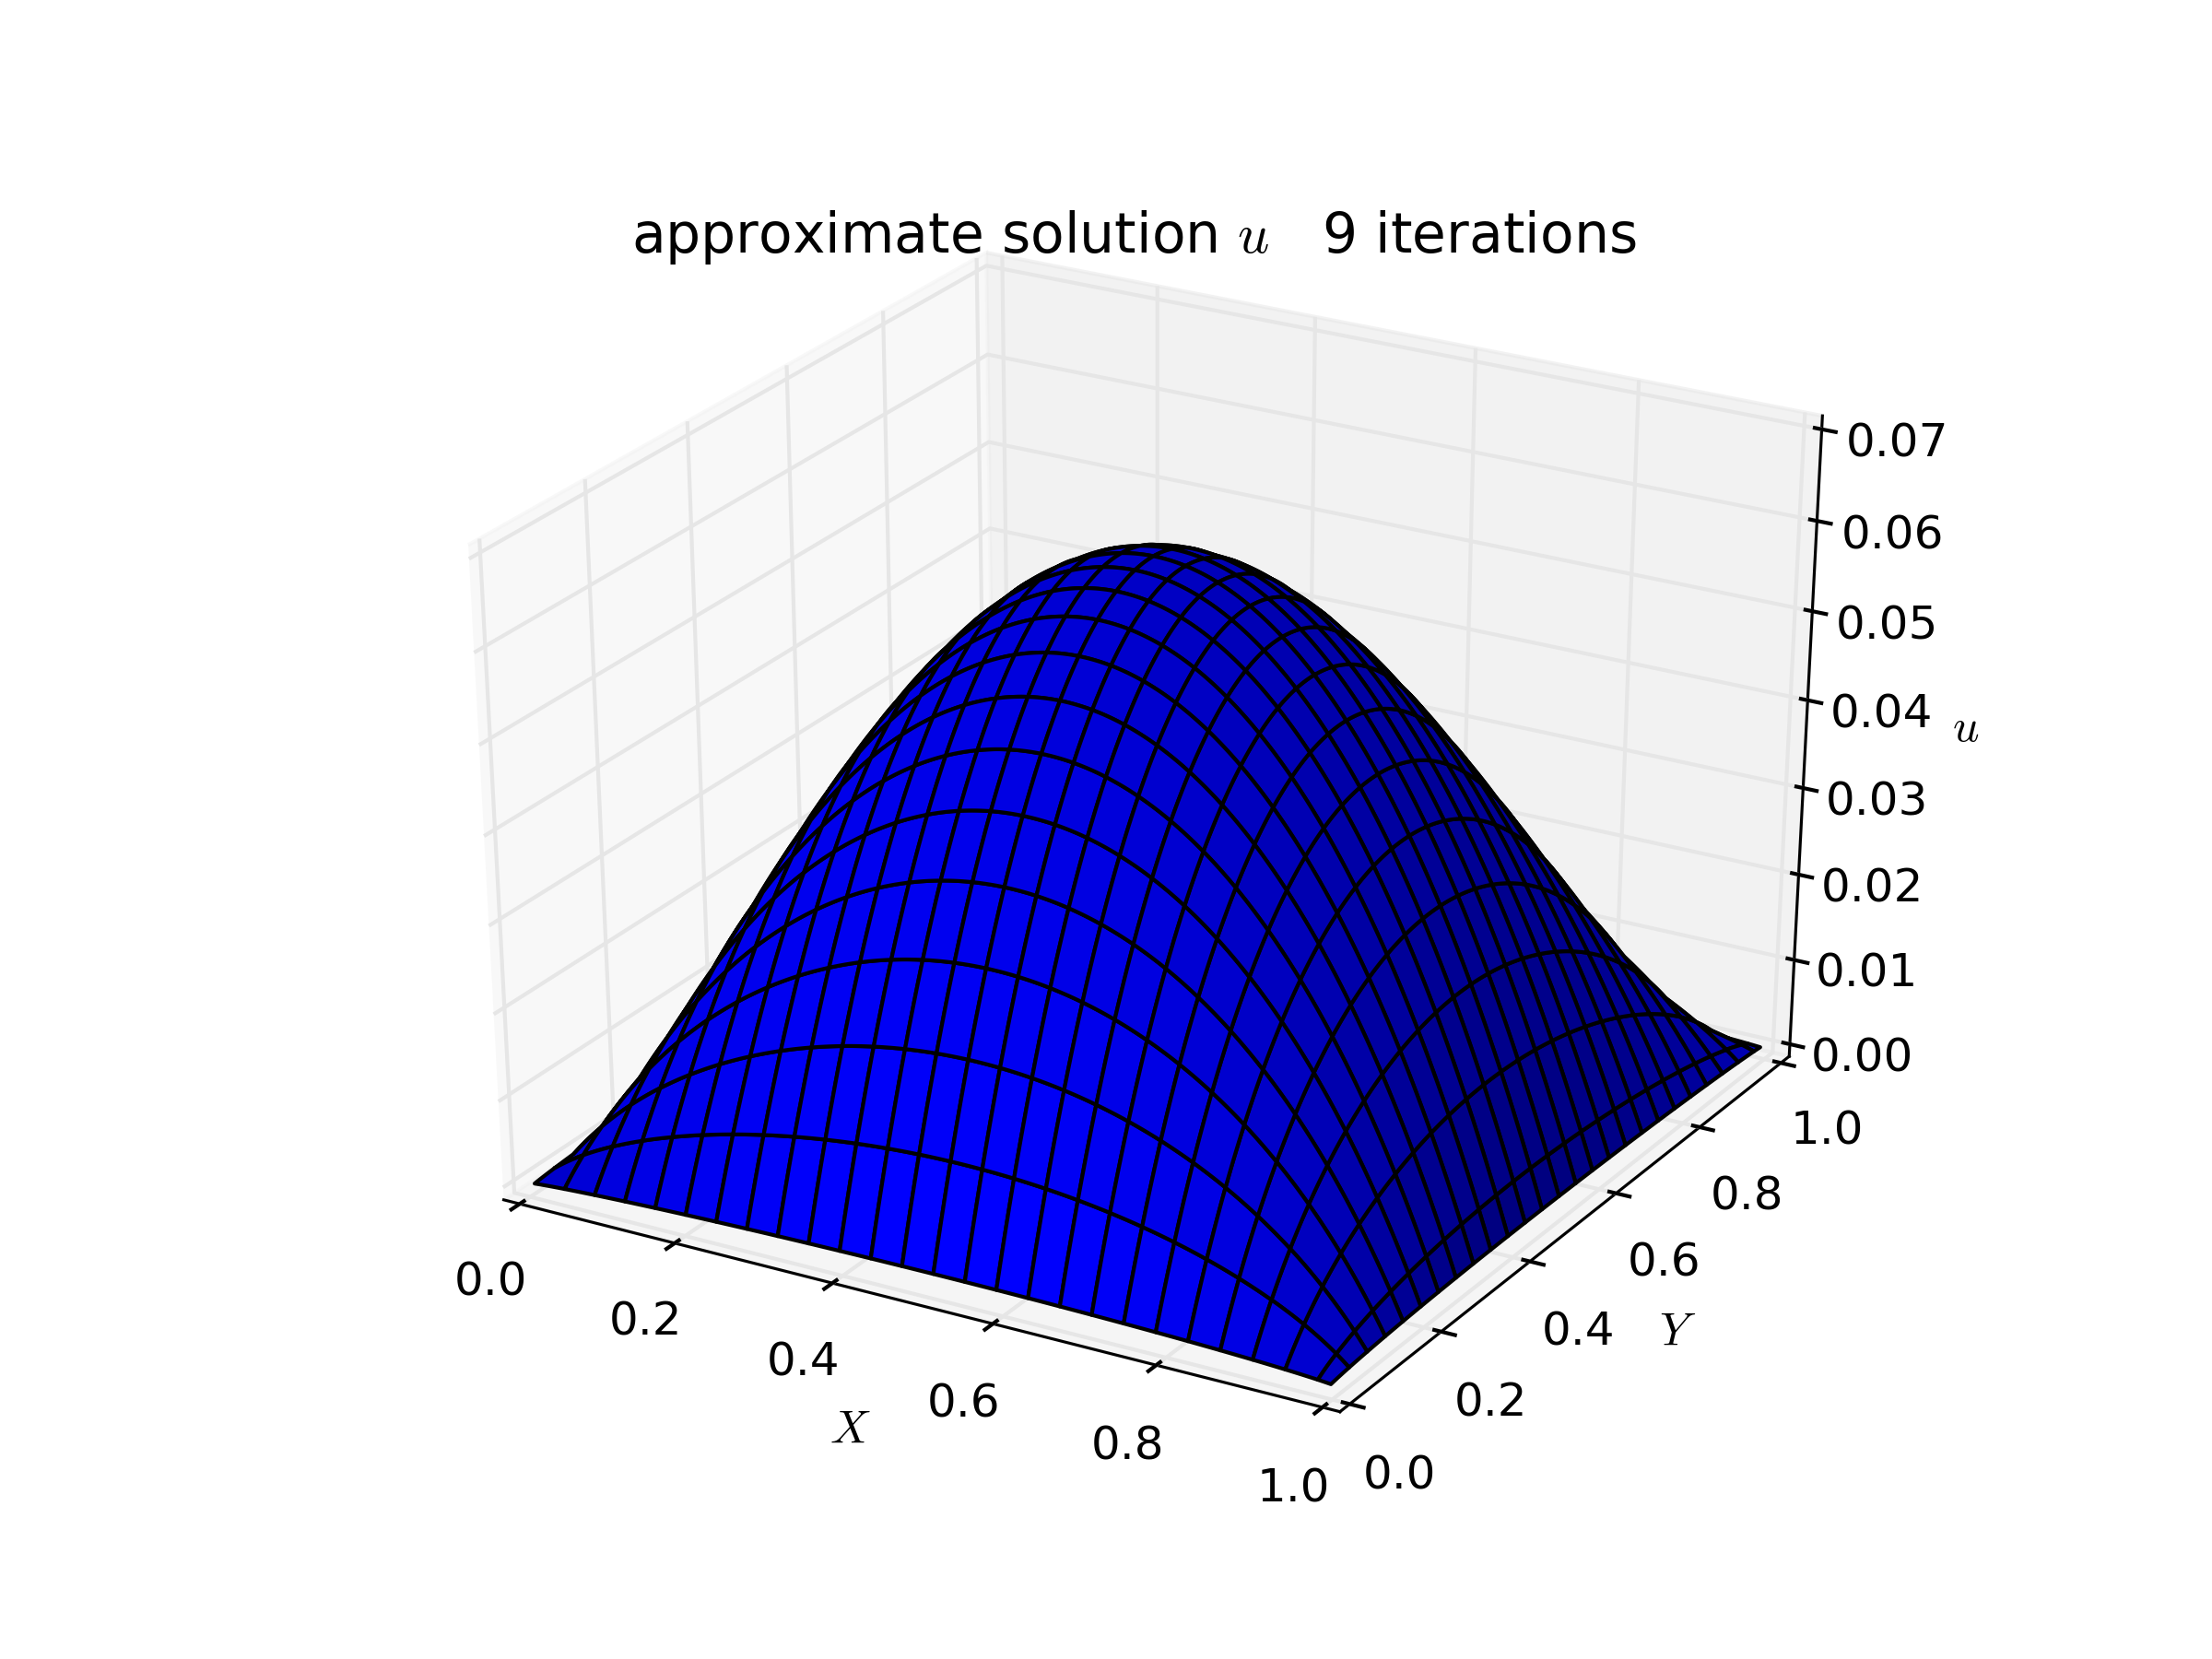
\includegraphics[width=\textwidth]{figures/p1_run1_1.png}
        \caption*{solution, azimuth$=-60$}
    \end{subfigure}
    \hfill
    \begin{subfigure}[b]{0.45\textwidth}
        \centering
        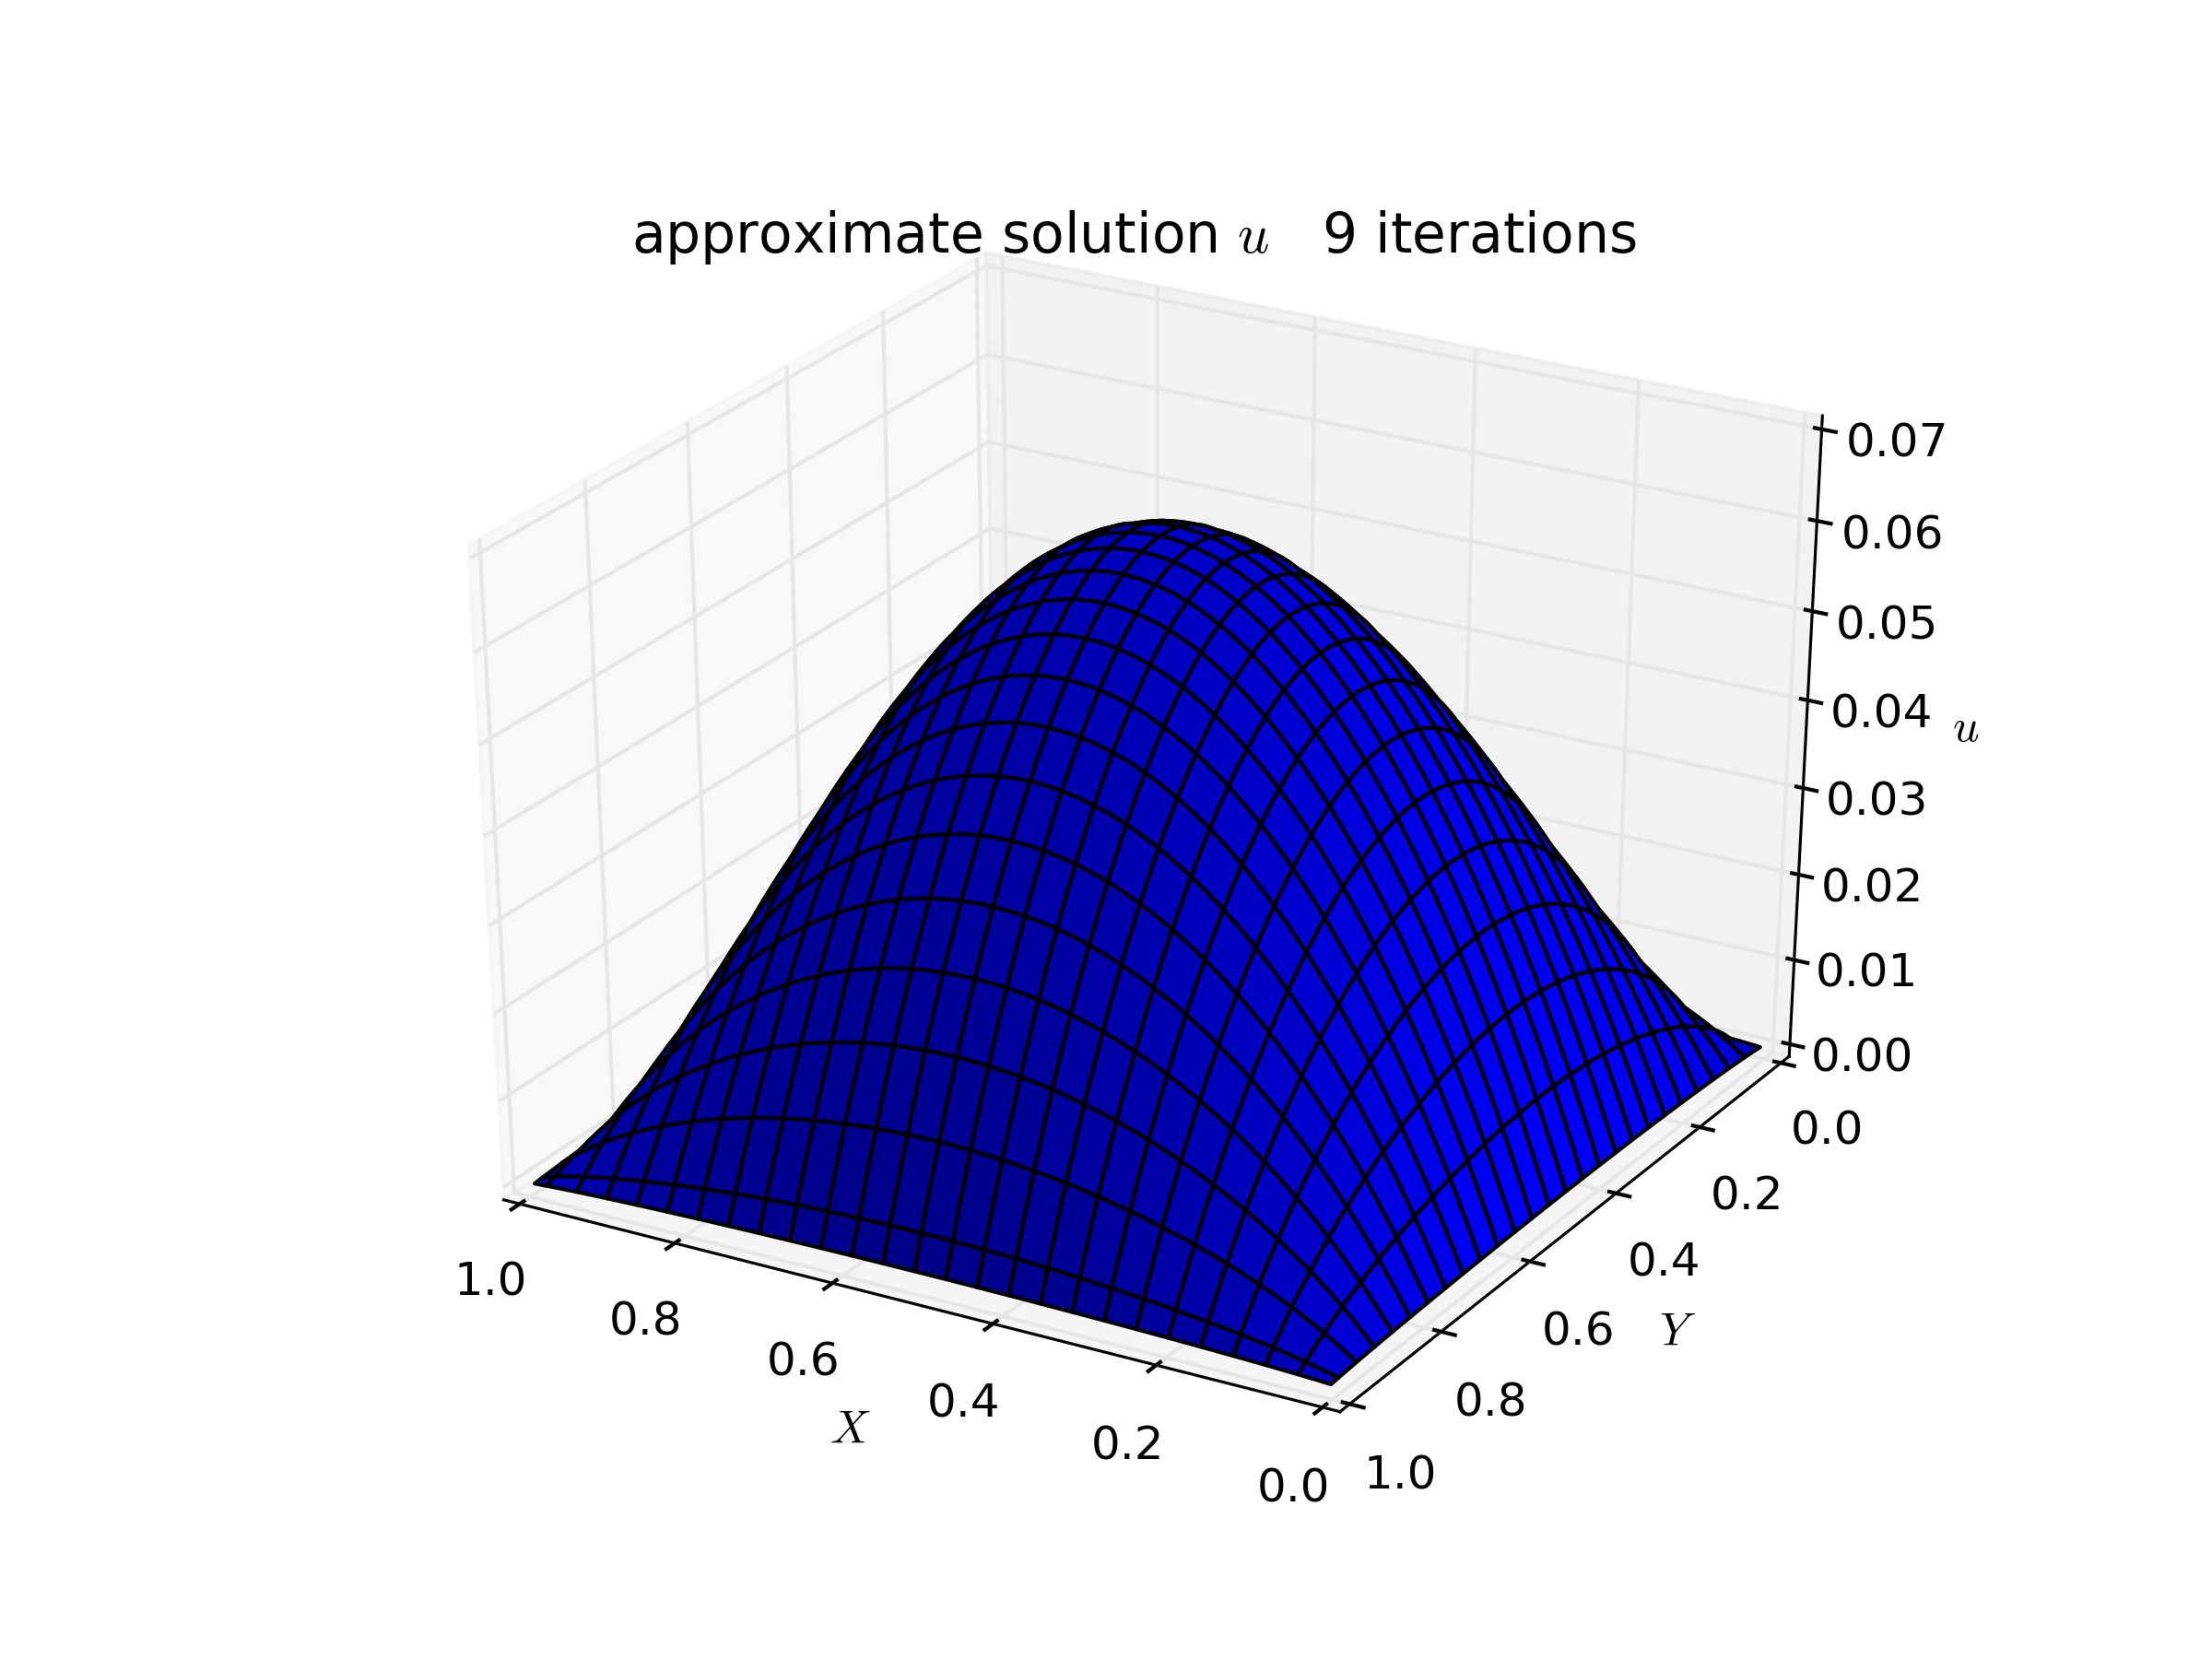
\includegraphics[width=\textwidth]{figures/p1_run1_2.png}
        \caption*{solution, azimuth$=120$}
    \end{subfigure}
    \hfill
    \begin{subfigure}[b]{0.45\textwidth}
        \centering
        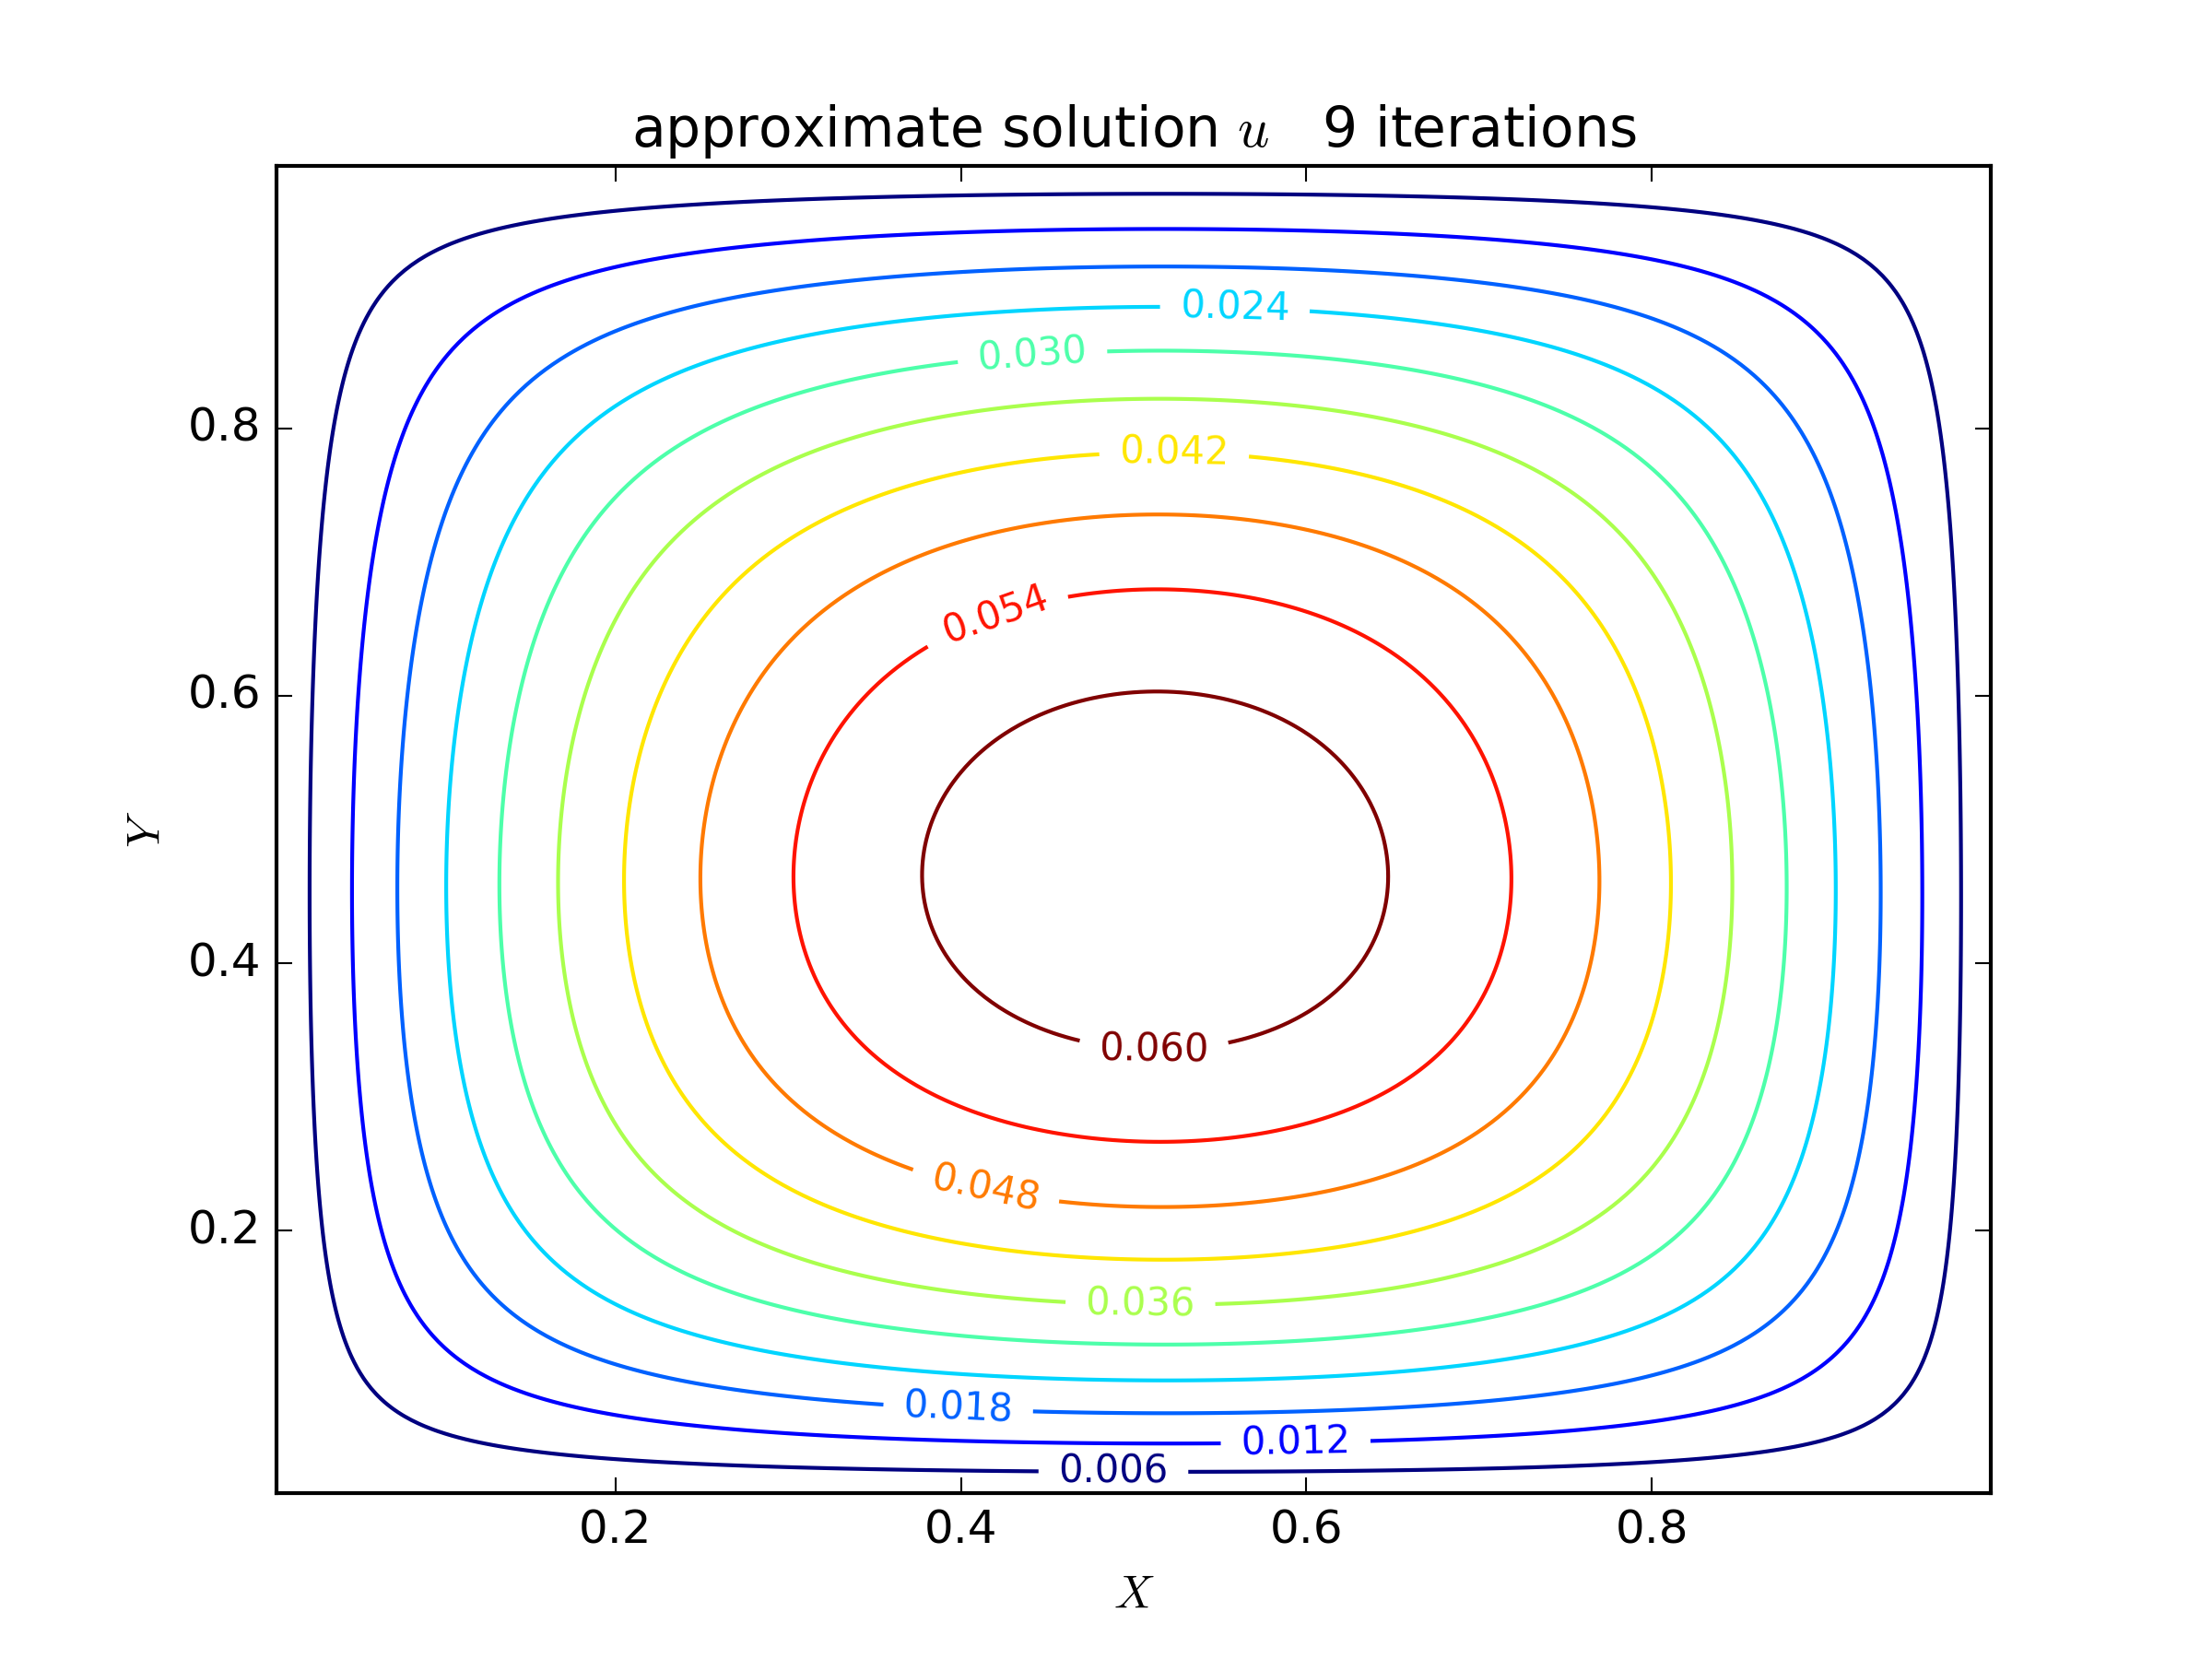
\includegraphics[width=\textwidth]{figures/p1_run1_4.png}
        \caption*{solution contour}
    \end{subfigure}
    \hfill
    \begin{subfigure}[b]{0.45\textwidth}
        \centering
        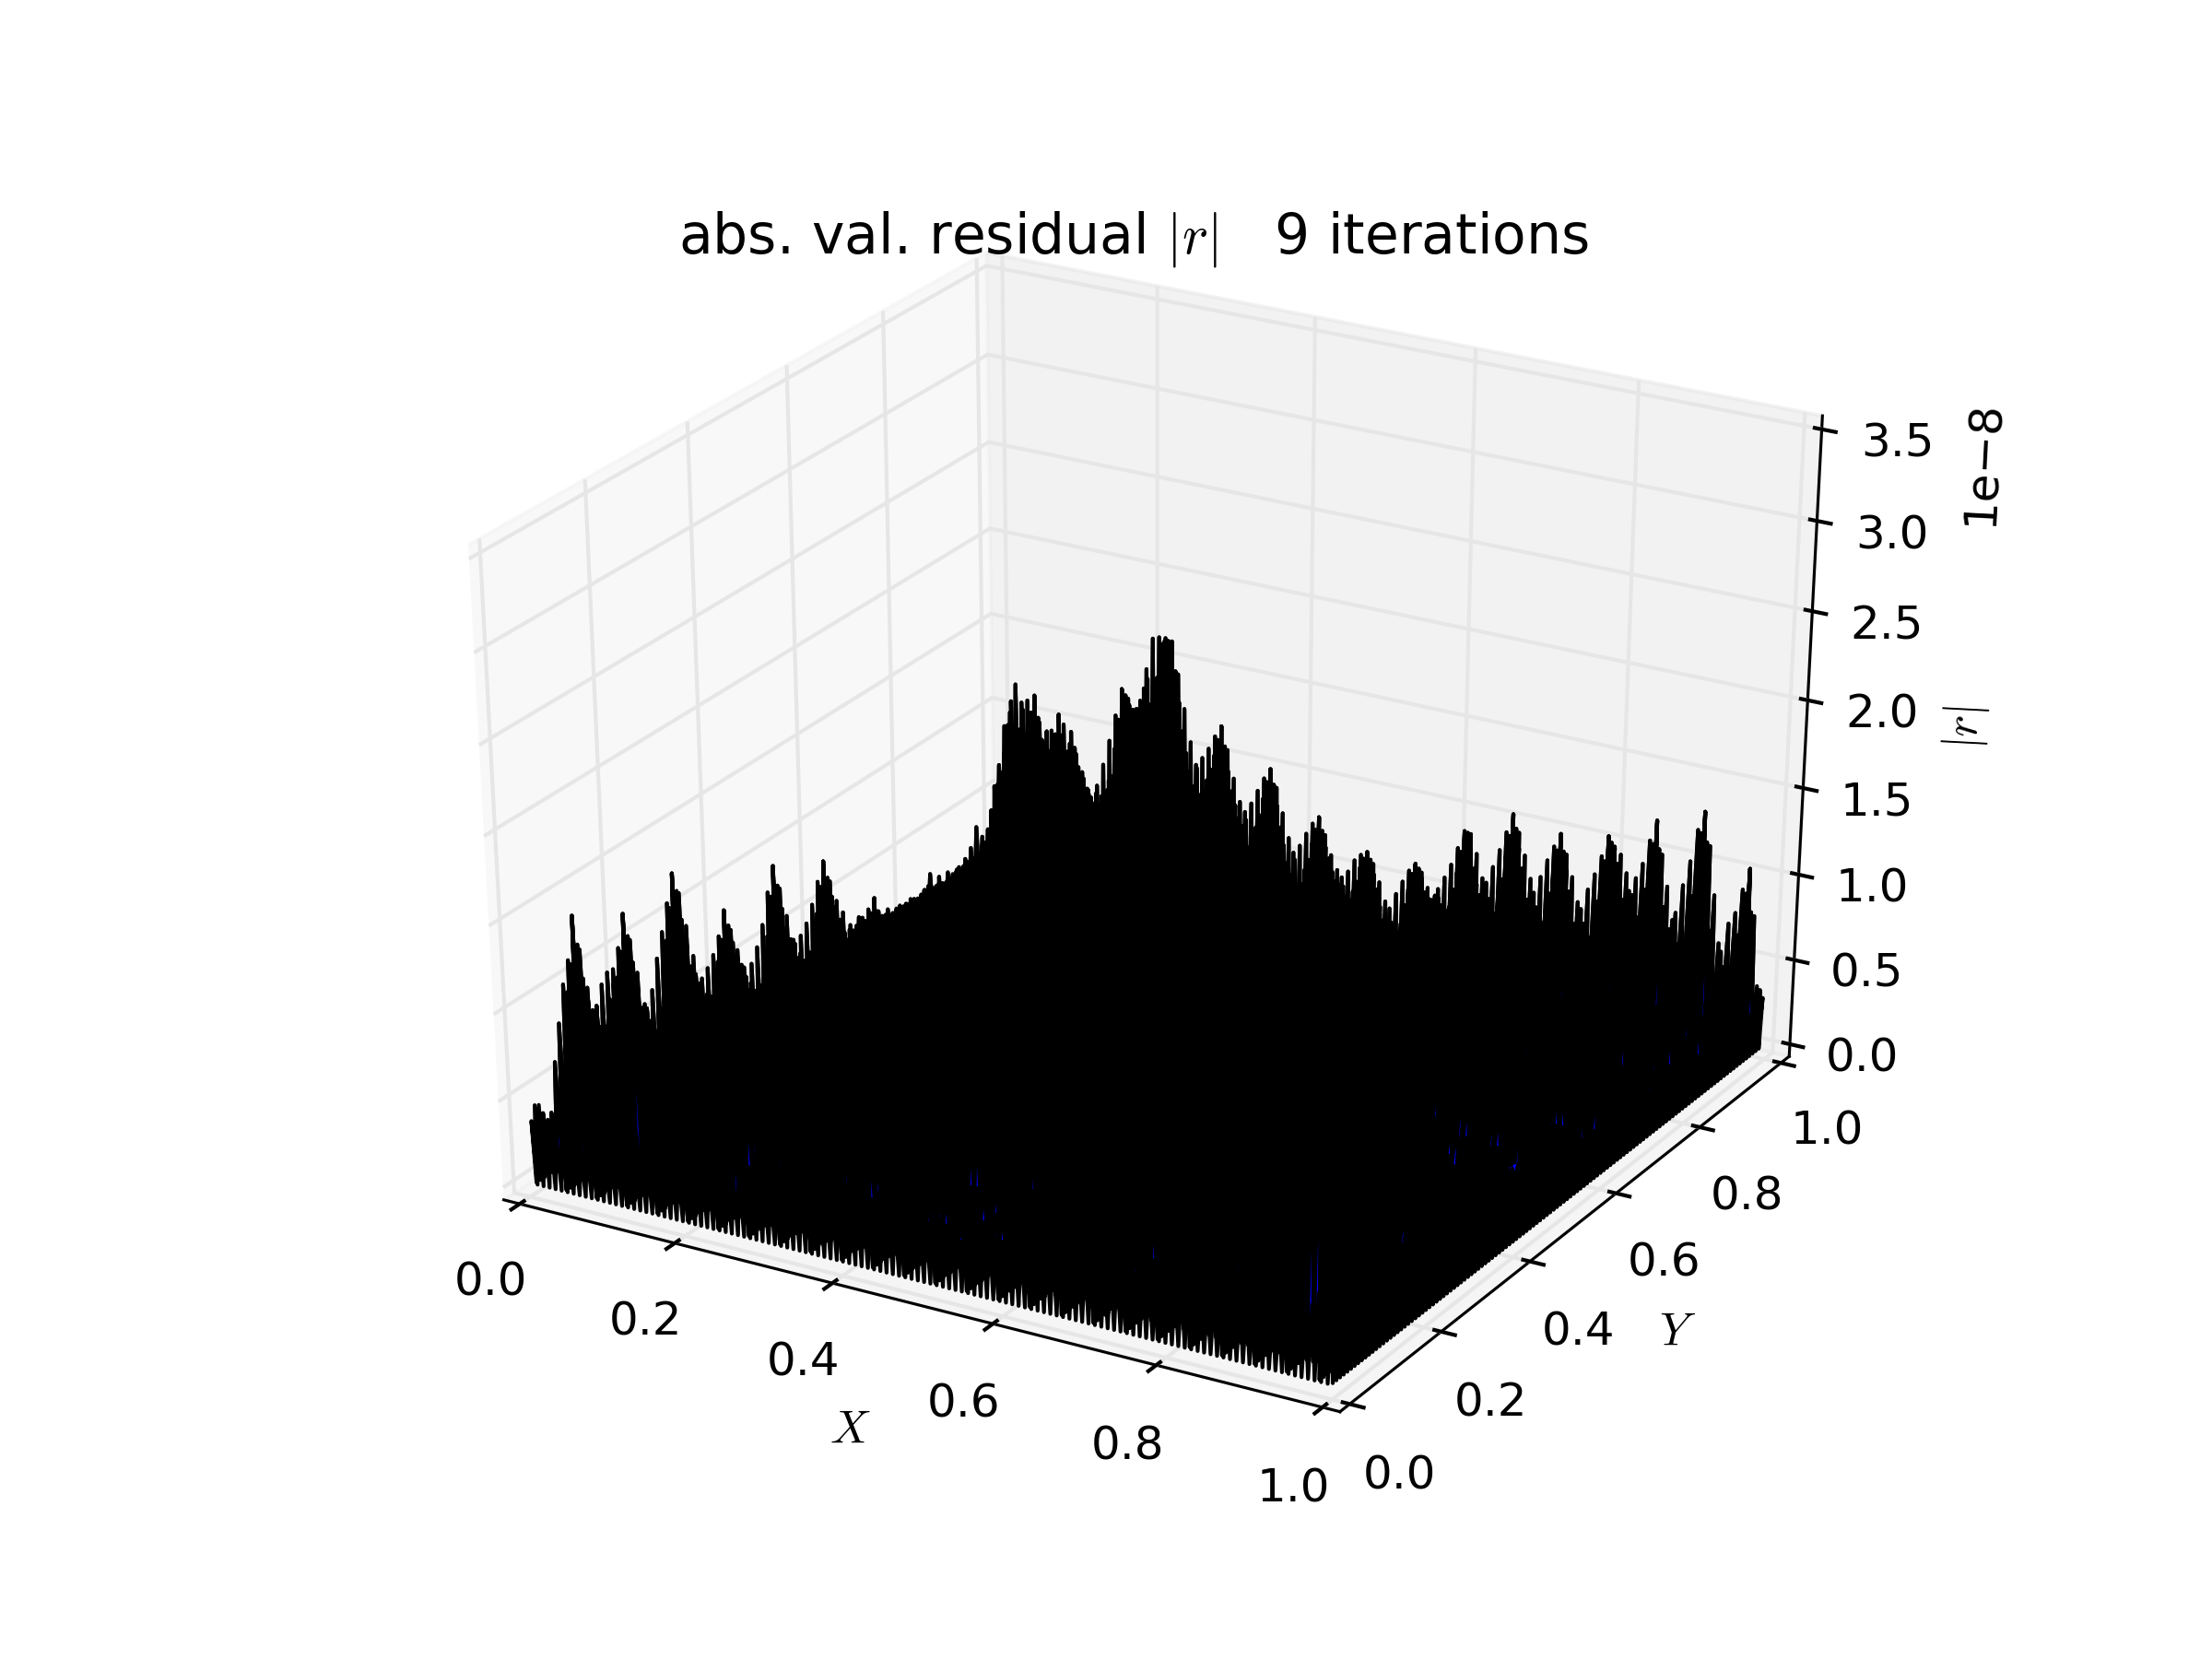
\includegraphics[width=\textwidth]{figures/p1_run1_3.png}
        \caption*{absolute value of the residual}
    \end{subfigure}
    \caption*{The above simulation was run with relative tolerance $10^{-7}$, $h=2^{-8}$, $\nu_1 = \nu_2 = 1$, and took $9$ iterations to converge.  Top row: approximate solution $u$ from two different views (note the $X$ and $Y$ axes).  Bottom Left: approximate solution contour plot.  Bottom right: The residual of the approximate solution (note the residual is on the order of $10^{-8}$).}
\end{figure}
\begin{table}[ht!]
    \centering
    \begin{tabular}{||l|l|l||}
        \hline\hline
        $k$ & $\norm{r_k}_\infty$ & $\dfrac{\vphantom{\frac{1}{1}}\norm{r_k}_\infty}{\vphantom{\frac{1}{1}}\norm{r_{k-1}}_\infty}$   \\
        \hline\hline
        1 & 0.368102 & - \\\hline
        2 & 0.0487561 & 0.132452981403 \\\hline
        3 & 0.00636013 & 0.130447720916 \\\hline
        4 & 0.0008433 & 0.132591695754 \\\hline
        5 & 0.00011053 & 0.131068270613 \\\hline
        6 & 1.43467e-05 & 0.129798992138 \\\hline
        7 & 1.84936e-06 & 0.128905142346 \\\hline
        8 & 2.37102e-07 & 0.128207510041 \\\hline
        9 & 3.02627e-08 & 0.127635734106 \\
        \hline\hline
    \end{tabular}
    \caption*{The above table shows the relative residuals of the above simulation.  We see $\approx87\%$ reduction in residual each iteration.  In the next simulation, we will change $\nu_1$ and get better convergence.}
\end{table}
\FloatBarrier
\begin{figure}[!htb]
    \centering
    \begin{subfigure}[b]{0.45\textwidth}
        \centering
        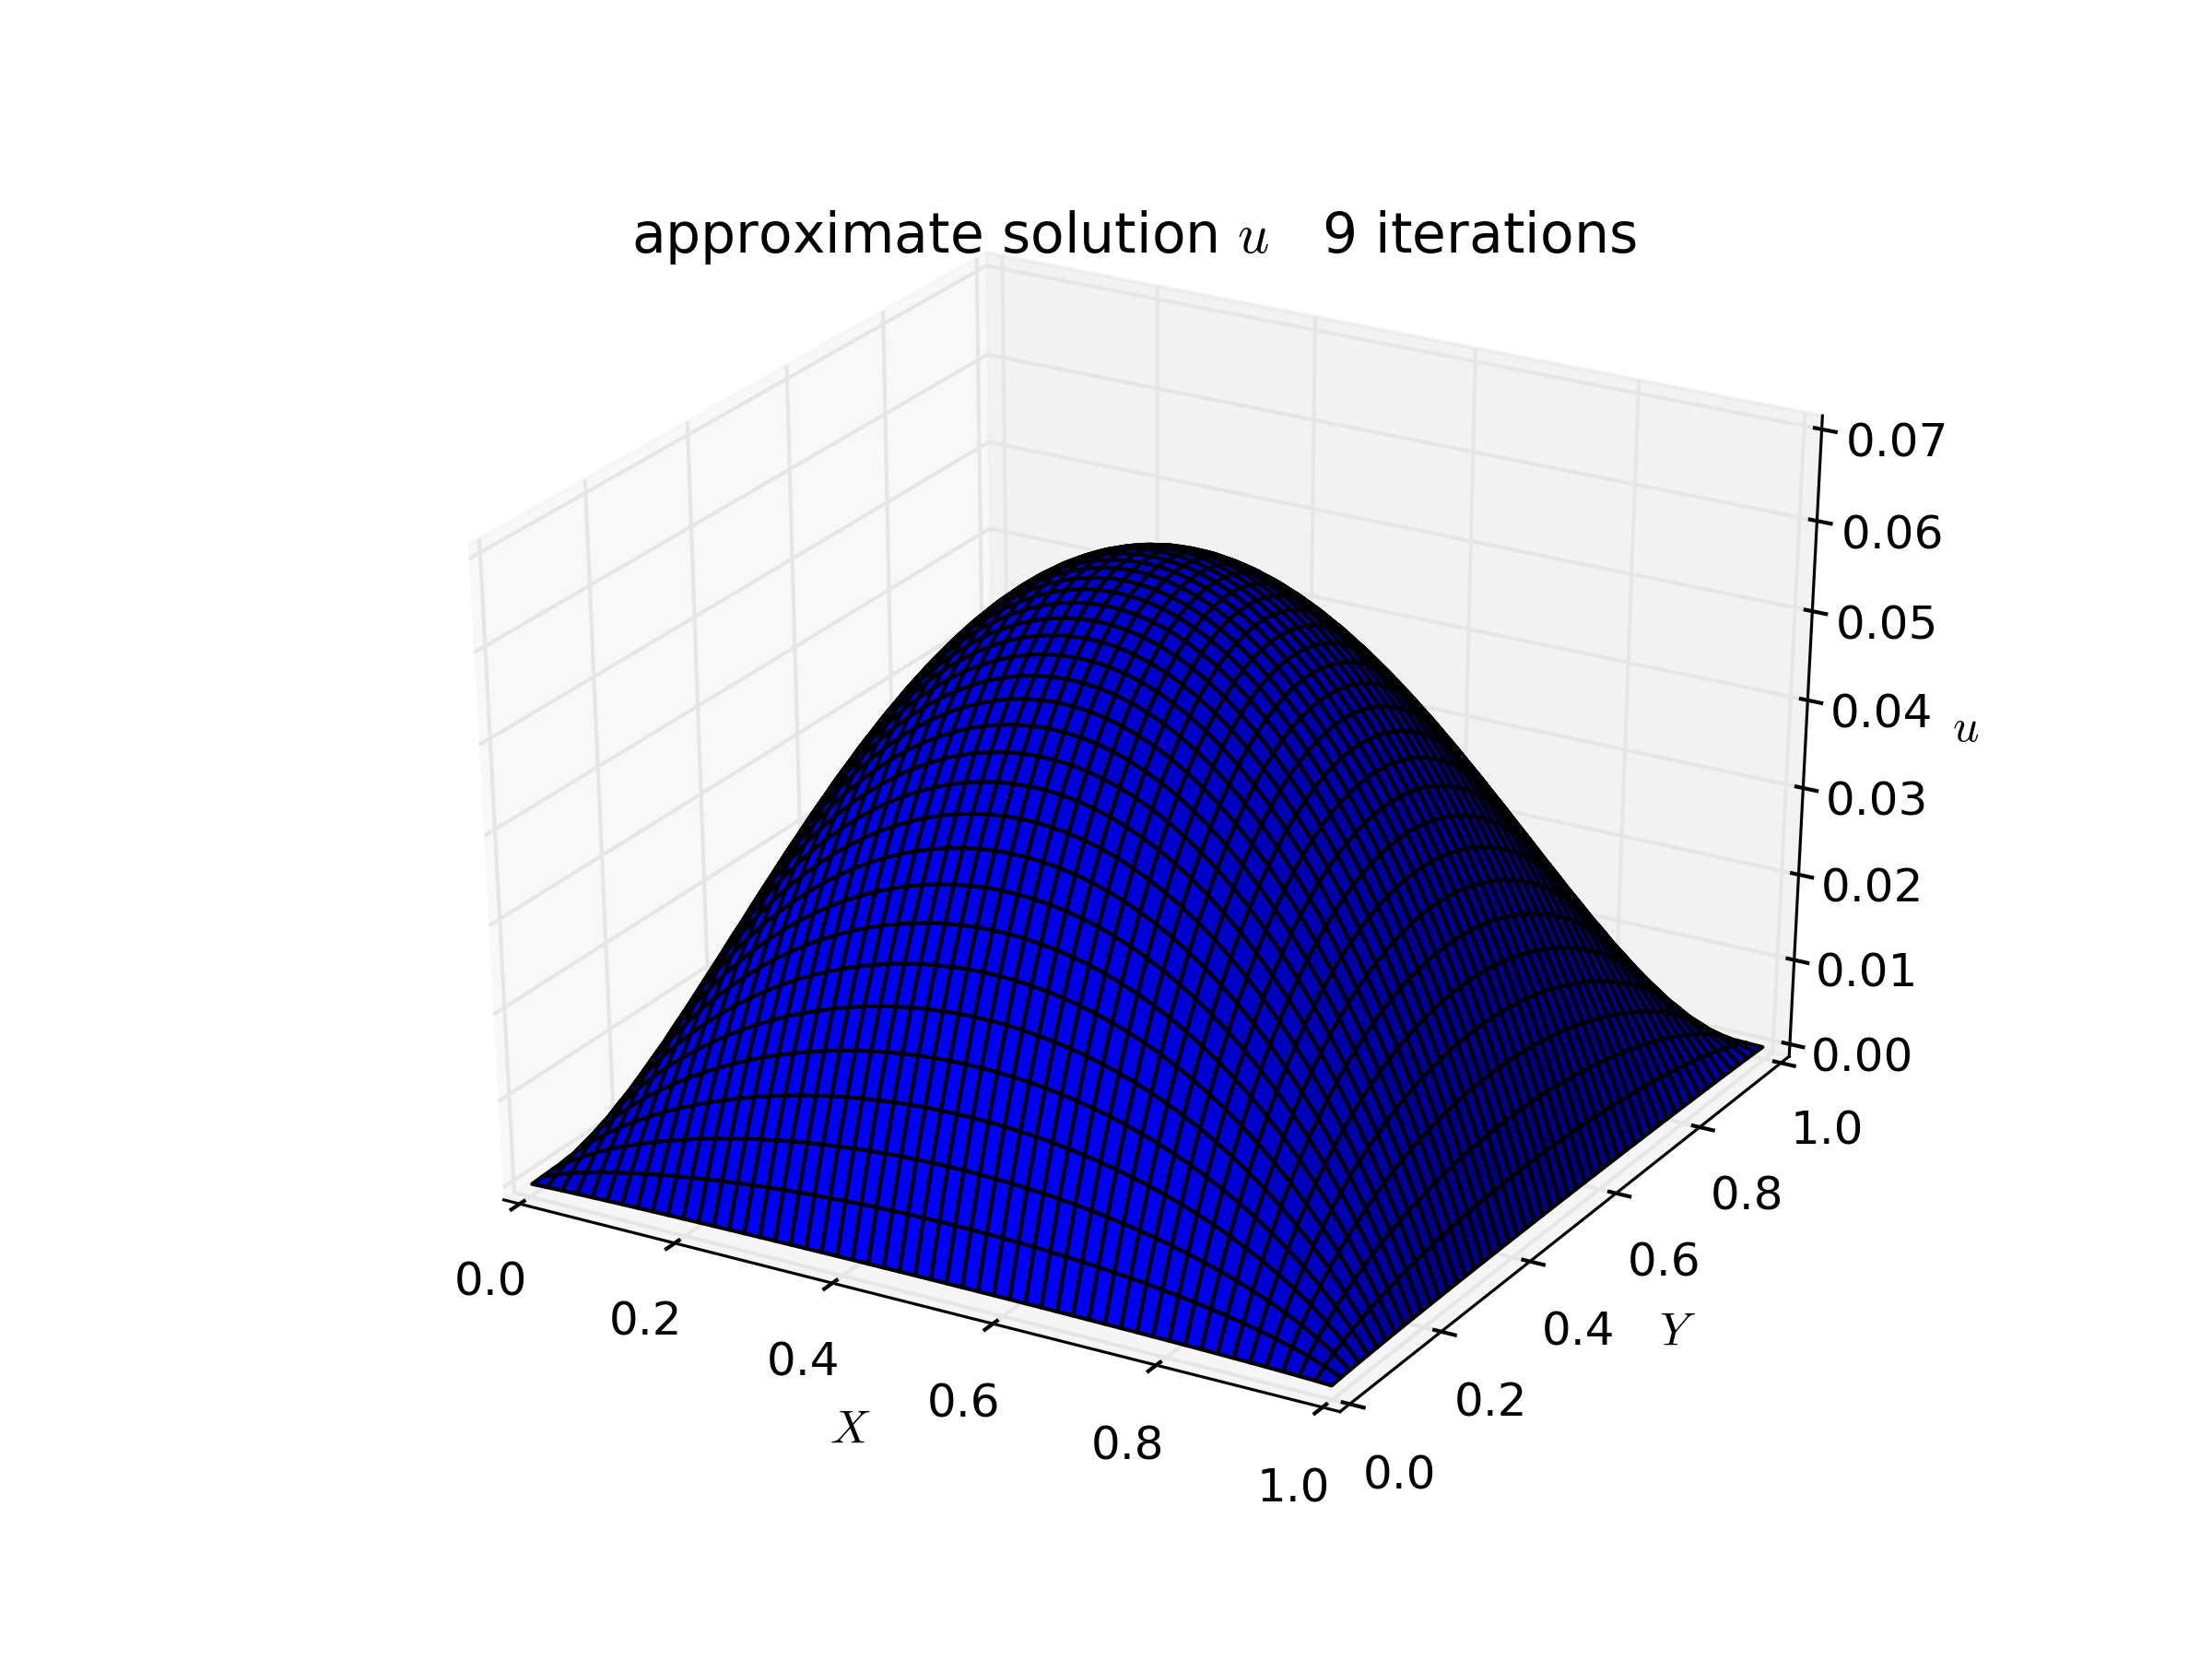
\includegraphics[width=\textwidth]{figures/p1_run2_1.png}
        \caption*{solution, azimuth$=-60$}
    \end{subfigure}
    \hfill
    \begin{subfigure}[b]{0.45\textwidth}
        \centering
        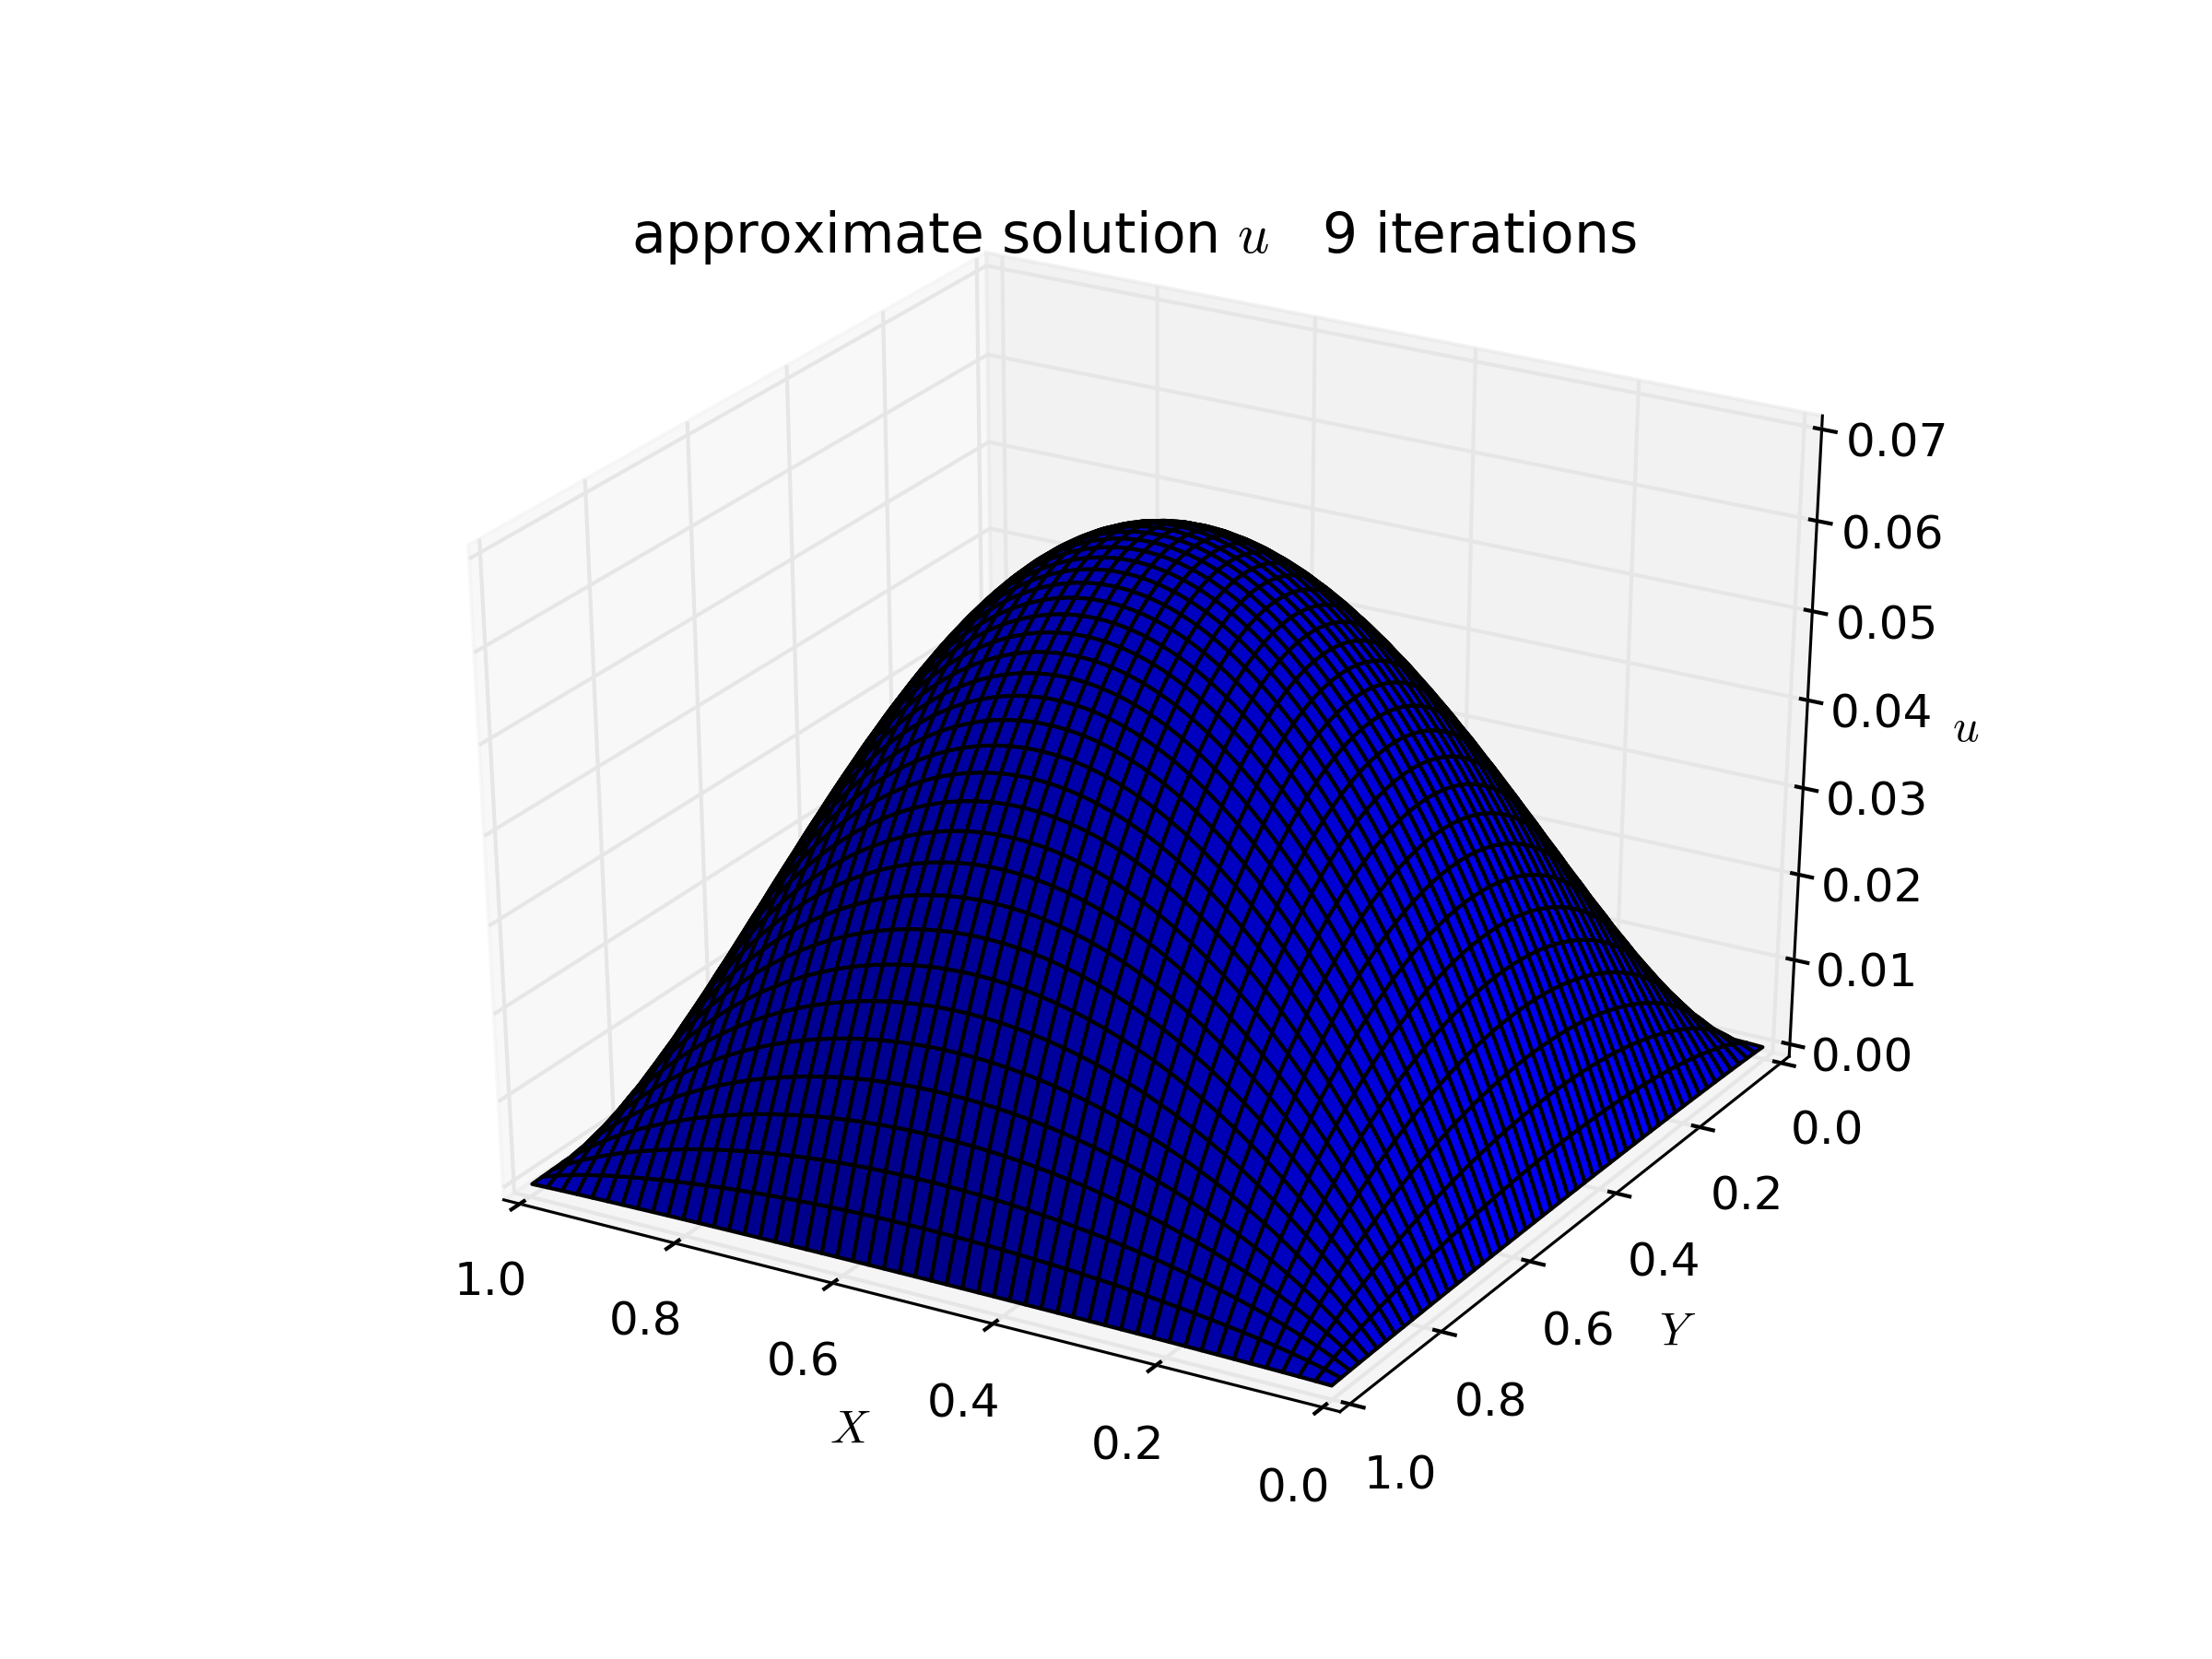
\includegraphics[width=\textwidth]{figures/p1_run2_2.png}
        \caption*{solution, azimuth$=120$}
    \end{subfigure}
    \hfill
    \begin{subfigure}[b]{0.45\textwidth}
        \centering
        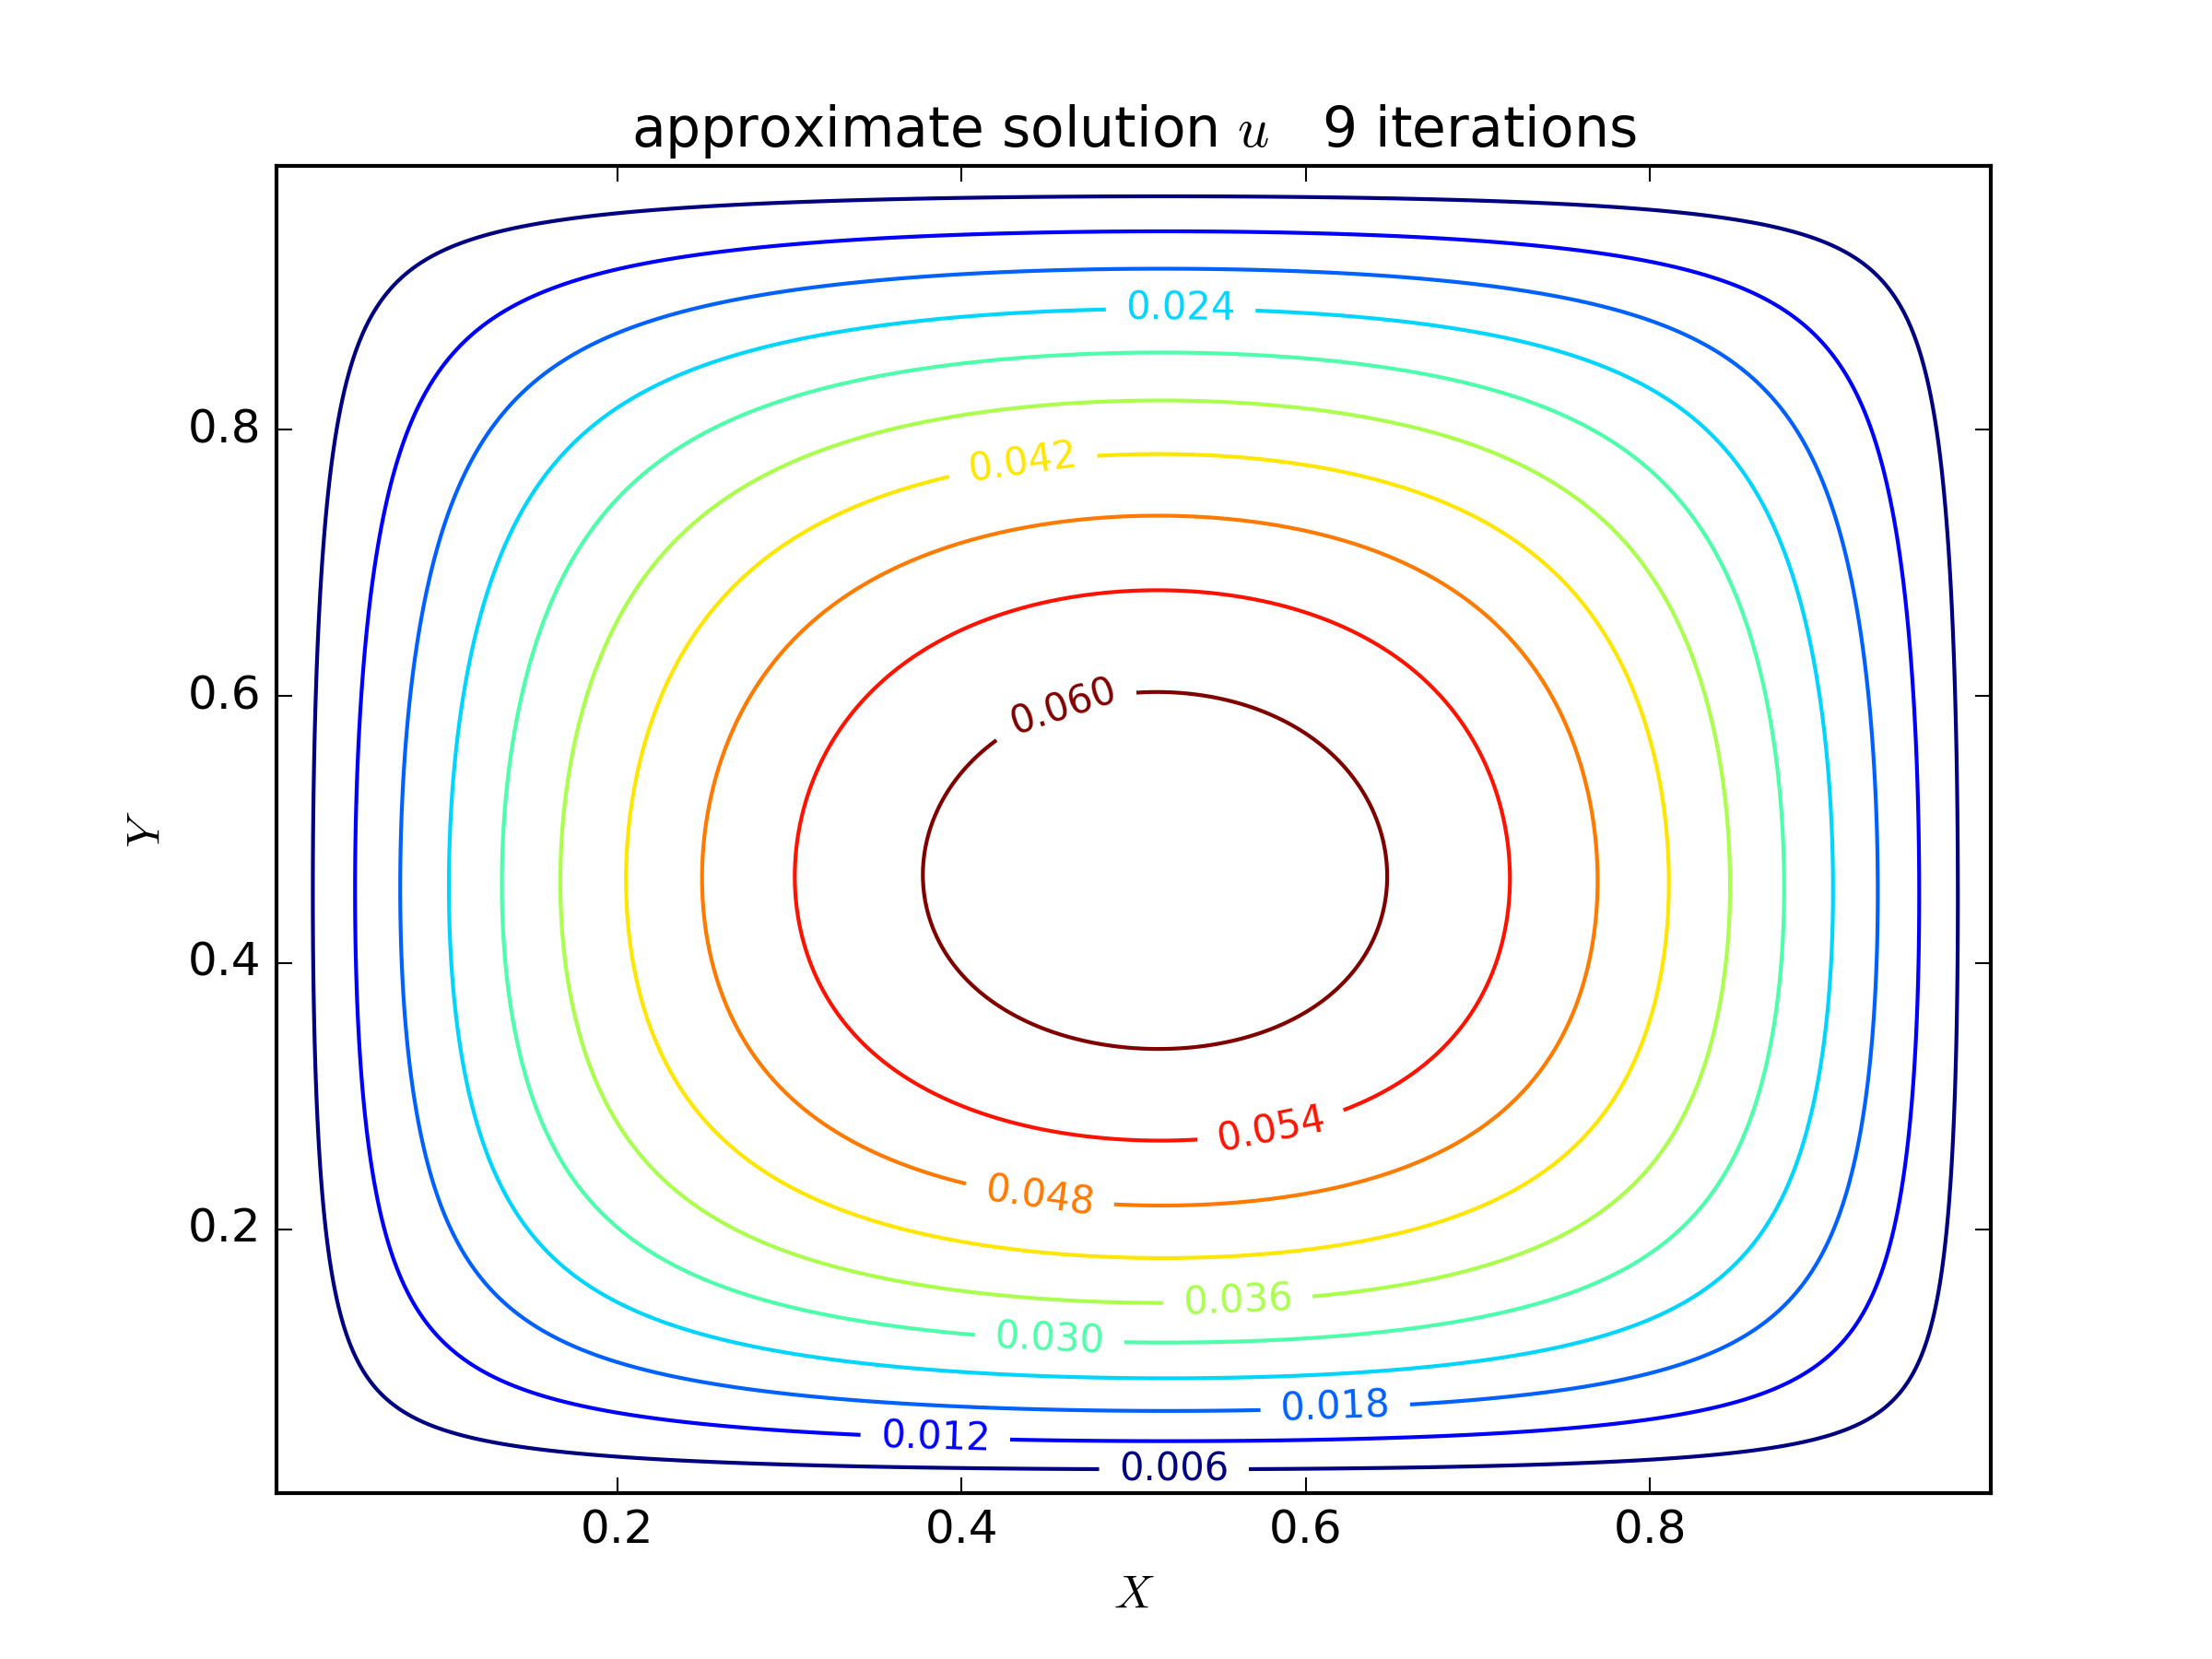
\includegraphics[width=\textwidth]{figures/p1_run2_4.png}
        \caption*{solution contour}
    \end{subfigure}
    \hfill
    \begin{subfigure}[b]{0.45\textwidth}
        \centering
        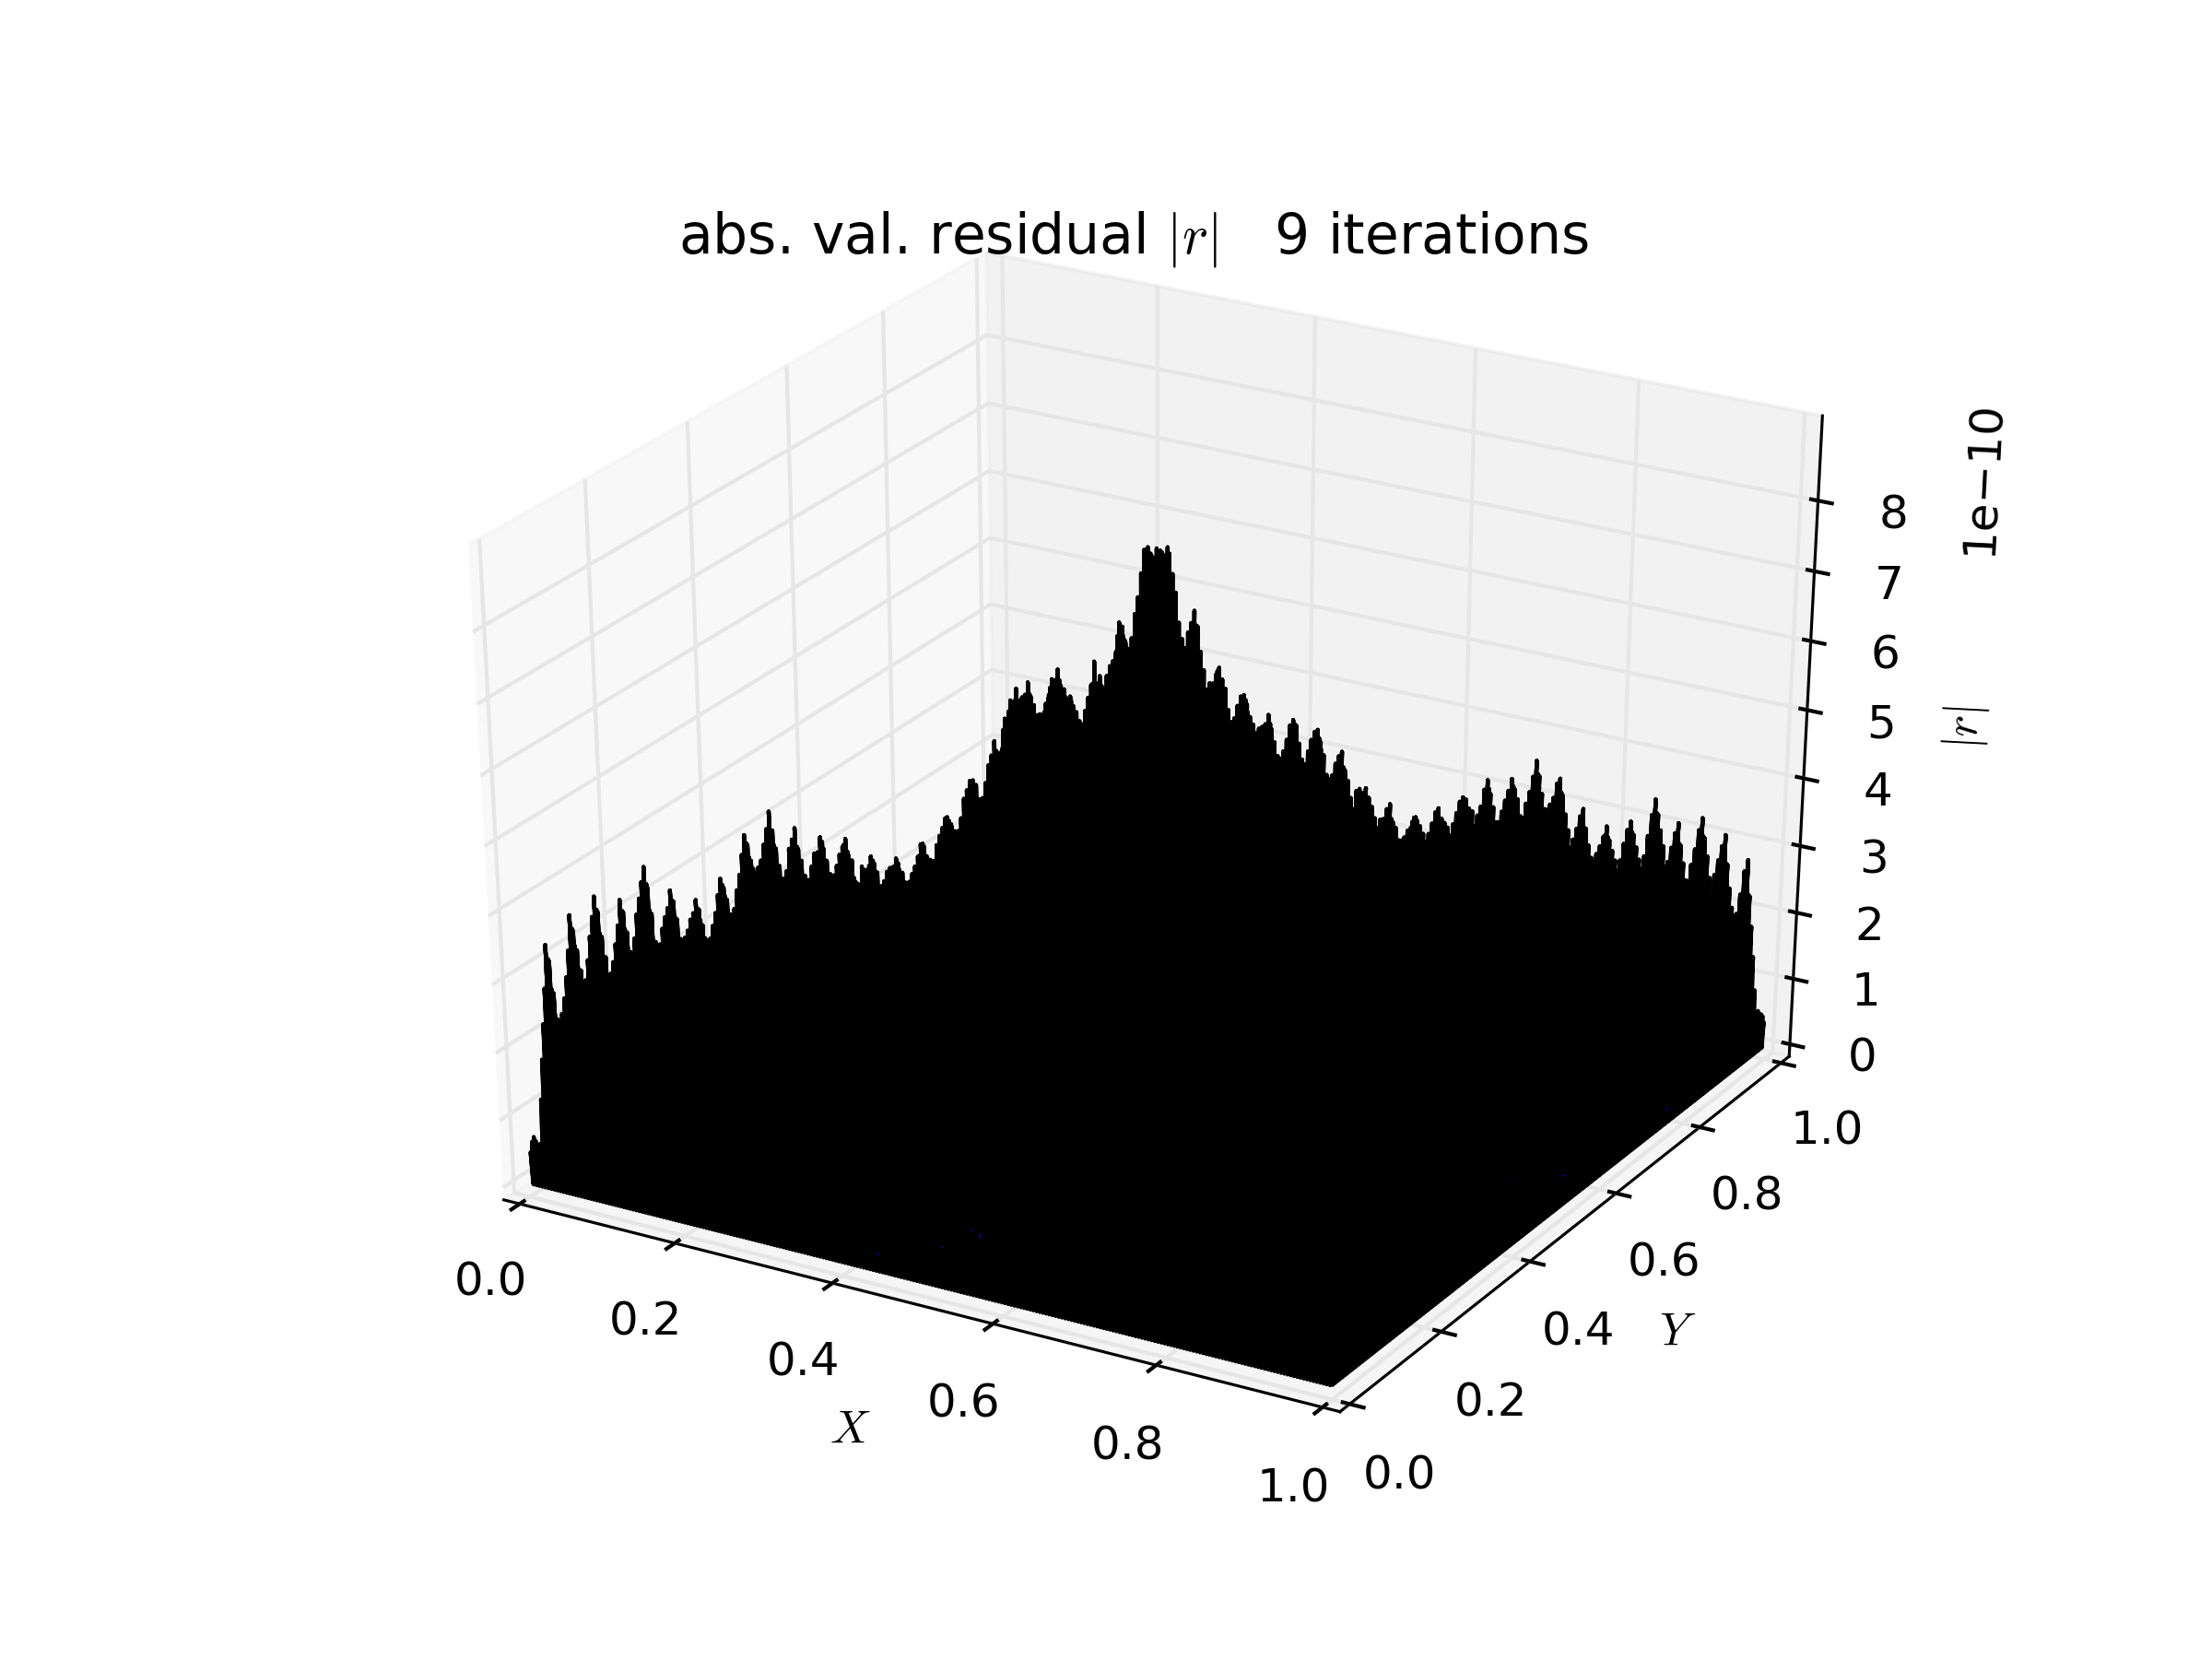
\includegraphics[width=\textwidth]{figures/p1_run2_3.png}
        \caption*{absolute value of the residual}
    \end{subfigure}
    \caption*{This simulation was run with relative tolerance $10^{-9}$, $h=2^{-9}$, $\nu_1 = 2$, $\nu_2 = 1$, and took $9$ iterations to converge.  Note the residual is on the order of $10^{-10}$.}
\end{figure}
\begin{table}[ht!]
    \centering
    \begin{tabular}{||l|l|l||}
        \hline\hline
        $k$ & $\norm{r_k}_\infty$ & $\dfrac{\vphantom{\frac{1}{1}}\norm{r_k}_\infty}{\vphantom{\frac{1}{1}}\norm{r_{k-1}}_\infty}$   \\
        \hline\hline
        1 & 0.242426    & -                               \\\hline
        2 & 0.0222294   & 0.0916957149997                 \\\hline
        3 & 0.00198422  & 0.0892610393309                 \\\hline
        4 & 0.000174193 & 0.0877893609761                 \\\hline
        5 & 1.52764e-05 & 0.0876981172233                 \\\hline
        6 & 1.34612e-06 & 0.0881171180771                 \\\hline
        7 & 1.1793e-07  & 0.0876074906573                 \\\hline
        8 & 1.03002e-08 & 0.087341465529                  \\\hline
        9 & 8.88707e-10 & 0.0862809077436                 \\\hline
    \hline
    \end{tabular}
    \caption*{The above table shows the relative residuals of the above simulation.  We see $\approx91\%$ reduction in residual each iteration.}
\end{table}
\FloatBarrier
The following table shows the work needed to solve this system for $h = 2^{-6}$ and $\text{tol} = 10^{-6}$.
\begin{table}[ht!]
    \centering
    \begin{tabular}{||l|l|l|l||}
        \hline\hline
        Method & Iterations & Work per Iteration & Total Work \\
        \hline\hline
        SOR & 144 & 1 work unit & 144 work units \\\hline
        MG $(\nu_1,\nu_2) = (1,1)$ & 8 & $\frac{\vphantom{\frac{1}{1}}4}{3\vphantom{\frac{1}{1}}}\qty(2 + 4)$ work units & 64 work units\\\hline
        MG $(\nu_1,\nu_2) = (2,1)$ & 7 & $\frac{\vphantom{\frac{1}{1}}4}{3\vphantom{\frac{1}{1}}}\qty(3 + 4)$ work units & 65 work units\\\hline
        MG $(\nu_1,\nu_2) = (2,2)$ & 6 & $\frac{\vphantom{\frac{1}{1}}4}{3\vphantom{\frac{1}{1}}}\qty(4 + 4)$ work units & 64 work units\\\hline\hline
    \end{tabular}
\end{table}
\FloatBarrier
and the following table shows the work needed to solve this system for $h = 2^{-8}$ and $\text{tol} = 10^{-7}$.
\begin{table}[ht!]
    \centering
    \begin{tabular}{||l|l|l|l||}
        \hline\hline
        Method & Iterations & Work per Iteration & Total Work \\
        \hline\hline
        SOR & 658 & 1 work unit & 658 work units \\\hline
        MG $(\nu_1,\nu_2) = (1,1)$ & 9 & $\frac{\vphantom{\frac{1}{1}}4}{3\vphantom{\frac{1}{1}}}\qty(2 + 4)$ work units & 72 work units\\\hline
        MG $(\nu_1,\nu_2) = (2,1)$ & 8 & $\frac{\vphantom{\frac{1}{1}}4}{3\vphantom{\frac{1}{1}}}\qty(3 + 4)$ work units & 75 work units\\\hline
        MG $(\nu_1,\nu_2) = (2,2)$ & 7 & $\frac{\vphantom{\frac{1}{1}}4}{3\vphantom{\frac{1}{1}}}\qty(4 + 4)$ work units & 75 work units\\\hline\hline
    \end{tabular}
\end{table}
\FloatBarrier
The work per iteration for the multigrid code is $\frac{4}{3}\qty(\nu_1 + \nu_2 + 4)$ where $4$ is for the computing the residual, restriction, interpolation, and correction.  Clearly the Multigrid code is desirable.









\FloatBarrier
\problem{Part II}{Choose \textbf{one} of the following problems.
\begin{itemize}
    \item[\ \ 2.] Numerically estimate the average convergence factor, $$\qty(\frac{\norm{e^{(k)}}_\infty}{\norm{e^{(0)}}_\infty})^{\nicefrac{1}{k}},$$ for different numbers of presmoothing steps, $\nu_1$, and postsmoothing steps, $\nu_2$, for $\nu = \nu_1 + \nu_2 \leq 4$.  Be sure to use a small value of $k$ because convergence may be reached very quickly.  What test problem did you use?  Do your results depend on the grid spacing?  Report the results in a table, and discuss which choices of $\nu_1$ and $\nu_2$ give the most efficient solver.
    \item[\ \ 3.] The multigrid V-cycle iteration is of the form $$u^{k+1} = (I - BA)u^k + Bf,$$ where $M = I - BA$ is the multigrid iteration matrix.  To compute the $k$th column of the multigrid iteration matrix, apply a single V-cycle to a problem with zero right-hand-side, $f$, and as an initial guess, $u^0$, that has a $1$ in the $k$th entry and zeros everywhere else.  For a small problem, e.g.~$h = 2^{-5}$ or $h = 2^{-6}$, form the multigrid matrix, compute the eigenvalues, and plot them in the complex plane.  Compute the spectral radius and $2$-norm of the multigrid iteration matrix for different numbers of presmoothing steps $\nu_1$, and postsmoothing steps, $\nu_2$.  Comment on your results.
\end{itemize}
}
\FloatBarrier

For the following tables, I am defining $E_k \coloneqq \qty(\frac{\norm{e^{(k)}}_\infty}{\norm{e^{(0)}}_\infty})^{\nicefrac{1}{k}}$.  To test this convergence rate, I initialized a random vector $u$, then passed it through the Laplacian $\laplacian$ to generate $f$.  Then I initialized a guess of $u_0 \equiv 0$ and ran the V-cycle code for a number of combinations of $\nu_1$ and $\nu_2$.  I solved the system numerically for $h = 2^{-i}$ for $i = 6,7,8,9$ and $\text{tol}=10^{-10}$.  The following four tables show the results for the four starting grid spacings.  The first two columns specify which values of $\nu$ used.  The third-seventh columns show the $E_1$-$E_5$.  The eighth column shows the number of iterations until convergence, and the ninth column shows the total time to completion.  Red entries are the smallest values in their respective columns, for a given $\nu=\nu_1+\nu_2$. \\

We see the best overall solver is $\nu_1 = \nu_2 = 1$.  Even though solvers with more smoothing steps have faster convergence with respect to a single iteration, each iteration takes longer, resulting in a slowdown.  In other words, the decrease in iteration count does not make up for the increase in smoothing time.  We also see that fast initial residual decrease does not necessarily mean it will converge first.  These results are independent of grid spacing.
\FloatBarrier
\begin{table}[ht!]
\centering
\begin{tabular}{||l|l|||l|l|l|l|l||l||l||}
\hline\hline
   $\nu_1$ &   $\nu_2$ &       $E_1$ &       $E_2$ &       $E_3$ &       $E_4$ &      $E_5$ &   iterations &     time \\
\hline\hline
      0 &      1 & 0.648938  & 0.43606   & 0.411233  & 0.399007  & 0.390484  &    {\color{red}19} & {\color{red}0.724328} \\\hline
      1 &      0 & {\color{red}0.487977}  & {\color{red}0.358102}  & {\color{red}0.347434}  & {\color{red}0.342882}  & {\color{red}0.340151}  &    21 & 0.804955 \\\hline\hline\hline

      0 &      2 & 0.357835  & 0.242341  & 0.225531  & 0.218747  & 0.2141    &    12 & 0.767544 \\\hline
      1 &      1 & {\color{red}0.116416}  & {\color{red}0.10496}   & {\color{red}0.107306}  & {\color{red}0.109805}  & {\color{red}0.112209}  &     {\color{red}9} & {\color{red}0.617404} \\\hline
      2 &      0 & 0.204627  & 0.180517  & 0.183596  & 0.184137  & 0.183818  &    13 & 0.879385 \\\hline\hline\hline

      0 &      3 & 0.278089  & 0.174162  & 0.156014  & 0.147177  & 0.141667  &    10 & 0.828848 \\\hline
      1 &      2 & {\color{red}0.0640793} & {\color{red}0.0687802} & {\color{red}0.0735935} & {\color{red}0.0760558} & {\color{red}0.077577}  &     {\color{red}8} & 0.664636 \\\hline
      2 &      1 & 0.0676902 & 0.0720939 & 0.076164  & 0.0780719 & 0.079116  &     {\color{red}8} & {\color{red}0.658428} \\\hline
      3 &      0 & 0.141664  & 0.126482  & 0.126586  & 0.125945  & 0.125153  &    11 & 0.93447  \\\hline\hline\hline

      0 &      4 & 0.232654  & 0.137391  & 0.119456  & 0.110986  & 0.106034  &     9 & 1.05532  \\\hline
      1 &      3 & 0.0465466 & {\color{red}0.053058}  & {\color{red}0.0563639} & {\color{red}0.0581954} & {\color{red}0.0592385} &     {\color{red}7} & 0.818631 \\\hline
      2 &      2 & {\color{red}0.0457535} & 0.0536427 & 0.0570361 & 0.0587056 & 0.0596329 &     {\color{red}7} & 0.73804  \\\hline
      3 &      1 & 0.0459446 & 0.0541799 & 0.0574189 & 0.0589796 & 0.0598539 &     {\color{red}7} & {\color{red}0.73296}  \\\hline
      4 &      0 & 0.108241  & 0.0995232 & 0.099261  & 0.0981586 & 0.0970414 &    10 & 1.03422  \\\hline\hline\hline
\end{tabular}
\caption*{$h=2^{-6}$, $\text{tol}=10^{-10}$}
\end{table}

\begin{table}[ht!]
\centering
\begin{tabular}{||l|l|||l|l|l|l|l||l||l||}
\hline\hline
   $\nu_1$ &   $\nu_2$ &       $E_1$ &       $E_2$ &       $E_3$ &       $E_4$ &      $E_5$ &   iterations &     time \\
\hline\hline
      0 &      1 & 0.70366   & 0.481388  & 0.429346  & 0.417088  & 0.408186  &    {\color{red}20} & {\color{red}3.32238} \\\hline
      1 &      0 & {\color{red}0.485865}  & {\color{red}0.362892}  & {\color{red}0.348612}  & {\color{red}0.345926}  & {\color{red}0.346277}  &    21 & 3.33875 \\\hline\hline\hline

      0 &      2 & 0.434735  & 0.276942  & 0.252261  & 0.237177  & 0.226658  &    12 & 3.77767 \\\hline
      1 &      1 & {\color{red}0.122205}  & {\color{red}0.106187}  & {\color{red}0.108739}  & {\color{red}0.110965}  & {\color{red}0.11267}   &     {\color{red}9} & {\color{red}2.35127} \\\hline
      2 &      0 & 0.235093  & 0.17992   & 0.18189   & 0.185694  & 0.187109  &    13 & 3.3626  \\\hline\hline\hline

      0 &      3 & 0.335241  & 0.198951  & 0.177639  & 0.164716  & 0.156347  &    10 & 3.50262 \\\hline
      1 &      2 & 0.0745486 & {\color{red}0.0726438} & {\color{red}0.07437}   & {\color{red}0.0761915} & {\color{red}0.0774869} &     {\color{red}8} & 2.77373 \\\hline
      2 &      1 & {\color{red}0.0734148} & 0.0731706 & 0.0759087 & 0.077723  & 0.0788225 &     {\color{red}8} & {\color{red}2.68093} \\\hline
      3 &      0 & 0.151107  & 0.124623  & 0.126975  & 0.1282    & 0.12819   &    11 & 3.7284  \\\hline\hline\hline

      0 &      4 & 0.275804  & 0.156577  & 0.137083  & 0.125968  & 0.119102  &     8 & 3.52157 \\\hline
      1 &      3 & 0.0565209 & 0.0550546 & {\color{red}0.0566352} & {\color{red}0.058069}  & {\color{red}0.0590243} &     {\color{red}7} & {\color{red}2.97657} \\\hline
      2 &      2 & {\color{red}0.05011}   & {\color{red}0.0543289} & 0.0568788 & 0.0583994 & 0.0593422 &     {\color{red}7} & 3.1198  \\\hline
      3 &      1 & 0.0513003 & 0.0548133 & 0.0570978 & 0.058626  & 0.0595583 &     {\color{red}7} & 3.09173 \\\hline
      4 &      0 & 0.104464  & 0.0981119 & 0.100041  & 0.100405  & 0.099938  &    10 & 4.3511  \\\hline\hline\hline
\end{tabular}
\caption*{$h=2^{-7}$, $\text{tol}=10^{-10}$}
\end{table}

\begin{table}[ht!]
\centering
\begin{tabular}{||l|l|||l|l|l|l|l||l||l||}
\hline\hline
   $\nu_1$ &   $\nu_2$ &       $E_1$ &       $E_2$ &       $E_3$ &       $E_4$ &      $E_5$ &   iterations &     time \\
\hline\hline
      0 &      1 & 0.706771  & 0.489336  & 0.445883  & 0.429412  & 0.420973  &    {\color{red}20} & {\color{red}12.6659} \\\hline
      1 &      0 & {\color{red}0.534644}  & {\color{red}0.390108}  & {\color{red}0.360545}  & {\color{red}0.35716}   & {\color{red}0.357252}  &    21 & 13.5175 \\\hline\hline\hline

      0 &      2 & 0.465575  & 0.293528  & 0.267626  & 0.253044  & 0.242728  &    12 & 12.1829 \\\hline
      1 &      1 & {\color{red}0.136665}  & {\color{red}0.113503}  & {\color{red}0.11083}   & {\color{red}0.112133}  & {\color{red}0.113674}  &     {\color{red}9} &  {\color{red}9.0864} \\\hline
      2 &      0 & 0.226812  & 0.187928  & 0.187011  & 0.191024  & 0.192129  &    13 & 14.2484 \\\hline\hline\hline

      0 &      3 & 0.364358  & 0.212581  & 0.187315  & 0.174013  & 0.164484  &    10 & 14.1303 \\\hline
      1 &      2 & 0.0754427 & {\color{red}0.0724907} & {\color{red}0.0746506} & {\color{red}0.0766038} & {\color{red}0.0779877} &     {\color{red}8} & 11.2709 \\\hline
      2 &      1 & {\color{red}0.0723146} & 0.0735791 & 0.076192  & 0.0781318 & 0.0792078 &     {\color{red}8} & {\color{red}10.9372} \\\hline
      3 &      0 & 0.150527  & 0.127825  & 0.129261  & 0.130377  & 0.131182  &    11 & 14.9868 \\\hline\hline\hline

      0 &      4 & 0.298608  & 0.172087  & 0.141158  & 0.129261  & 0.122096  &     8 & 13.7246 \\\hline
      1 &      3 & 0.0540812 & {\color{red}0.0543202} & {\color{red}0.0567906} & {\color{red}0.0583588} & {\color{red}0.0594019} &     {\color{red}7} & 12.2086 \\\hline
      2 &      2 & 0.0538676 & 0.0546608 & 0.0572044 & 0.0587821 & 0.0597278 &     {\color{red}7} & 12.1011 \\\hline
      3 &      1 & {\color{red}0.0519433} & 0.0548087 & 0.0573617 & 0.0590001 & 0.0599155 &     {\color{red}7} & {\color{red}12.0719} \\\hline
      4 &      0 & 0.108124  & 0.0997209 & 0.101444  & 0.102353  & 0.102668  &    10 & 17.1891 \\\hline\hline\hline
\end{tabular}
\caption*{$h=2^{-8}$, $\text{tol}=10^{-10}$}
\end{table}

\begin{table}[ht!]
\centering
\vspace{-5cm}
\begin{tabular}{||l|l|||l|l|l|l|l||l||l||}
\hline\hline
   $\nu_1$ &   $\nu_2$ &       $E_1$ &       $E_2$ &       $E_3$ &       $E_4$ &      $E_5$ &   iterations &     time \\
\hline\hline
      0 &      1 & 0.814503  & 0.506634  & 0.47523   & 0.460882  & 0.448367  &    {\color{red}20} & {\color{red}53.3505} \\\hline
      1 &      0 & {\color{red}0.552184}  & {\color{red}0.387626}  & {\color{red}0.371623}  & {\color{red}0.368553}  & {\color{red}0.367149}  &    22 & 57.5223 \\\hline\hline\hline

      0 &      2 & 0.474977  & 0.311891  & 0.274758  & 0.263955  & 0.255797  &    12 & 48.9866 \\\hline
      1 &      1 & {\color{red}0.138544}  & {\color{red}0.11245}   & {\color{red}0.1112}    & {\color{red}0.112476}  & {\color{red}0.114036}  &     {\color{red}9} & {\color{red}36.7199} \\\hline
      2 &      0 & 0.224892  & 0.189581  & 0.1904    & 0.190866  & 0.191885  &    13 & 52.9136 \\\hline\hline\hline

      0 &      3 & 0.374745  & 0.24126   & 0.198747  & 0.1787    & 0.169587  &    10 & 55.0487 \\\hline
      1 &      2 & {\color{red}0.0735864} & {\color{red}0.0725248} & {\color{red}0.0753096} & {\color{red}0.0771247} & {\color{red}0.0783378} &     {\color{red}8} & 44.2941 \\\hline
      2 &      1 & 0.0745542 & 0.0756904 & 0.0774981 & 0.0789767 & 0.079857  &     {\color{red}8} & {\color{red}44.0936} \\\hline
      3 &      0 & 0.148192  & 0.12764   & 0.129203  & 0.130529  & 0.131821  &    11 & 60.5826 \\\hline\hline\hline

      0 &      4 & 0.325174  & 0.199243  & 0.16092   & 0.144477  & 0.135421  &     8 & 56.1599 \\\hline
      1 &      3 & 0.0534238 & {\color{red}0.0550205} & {\color{red}0.057335}  & {\color{red}0.0587958} & {\color{red}0.0597648} &     {\color{red}7} & {\color{red}49.0491} \\\hline
      2 &      2 & {\color{red}0.0525316} & 0.0556535 & 0.0579426 & 0.0594209 & 0.060221  &     {\color{red}7} & 49.1172 \\\hline
      3 &      1 & 0.0536964 & 0.0562632 & 0.0582736 & 0.0596727 & 0.0604218 &     {\color{red}7} & 48.8892 \\\hline
      4 &      0 & 0.109677  & 0.0996846 & 0.101494  & 0.103119  & 0.103739  &    10 & 70.1302 \\\hline\hline\hline
\end{tabular}
\caption*{$h=2^{-9}$, $\text{tol}=10^{-10}$}
\end{table}






\end{document}









